\documentclass[a4paper,spanish]{paper} 
\usepackage[margin=2cm]{geometry}
\usepackage{graphicx}
\usepackage{lipsum}
\usepackage{xcolor}
\usepackage{booktabs}
\usepackage{fancyhdr}
\usepackage[most]{tcolorbox}
\usepackage[authoryear]{natbib}
\usepackage{fancyvrb}
\usepackage[section]{placeins}
%\usepackage{blindtext} %for dummy text. Can remove when used with real text.
\usepackage{tabu} %for tables

\usepackage [spanish]{babel}
\usepackage[utf8]{inputenc}
\selectlanguage{spanish}

\usepackage [autostyle, spanish = spanish]{csquotes}

\MakeOuterQuote{"}


\pagestyle{fancy}
\fancyhf{}
\rhead{Documentación}
\lhead{Covid19-UCM}
\rfoot{\thepage}


\linespread{1.3}


\title{Plataforma PCR-Covid19 UCM}
\subtitle{Documentación de la herramienta\\
\hfill
\includegraphics[height=2.5cm]{UCMlogo.png}
\vspace{-3cm}}
\author{Universidad Complutense de Madrid}
\institution{2020UCM}

%\renewcommand{\familydefault}{\sfdefault} %command to change font to sans-serif

\definecolor{blue(ryb)}{rgb}{0.01, 0.28, 1.0}


\begin{document} 
\vspace{-3.5cm}
\maketitle
\hrule \hrule
\medskip
\vspace{-0.2cm}

\begin{center}
\textbf{DOCUMENTACIÓN}
\end{center}
\vspace{-0.3cm}
\textbf{Herramienta:} PCR-Covid19 UCM\\
\textbf{Versión:} 1.0
\textbf{Fecha:} \today\\



\medskip
\hrule
\hspace{1cm}

PCR-Covid19 es una plataforma informática creada por la Universidad Complutense de Madrid para la gestión y seguimiento de muestras PCR en la identificación del coronavirus SARS-CoV-2. SARS-CoV-2 (en inglés, \textit{severe acute respiratory syndrome coronavirus}), un tipo de coronavirus causante de la enfermedad por coronavirus de 2019 (COVID-19) cuya expansión mundial ha provocado la pandemia de 2019-2020. Inicialmente llamado 2019-nCoV (en inglés, \textit{2019-novel coronavirus}).

%\blindtext[2]  %used for random text


\medskip
\begin{tcolorbox}[colback=blue!3!white,colframe=blue(ryb)!50!black,title=\textbf{Contenido}]

Este documento recoge la funcionalidad, manejo, y protocolo de uso de la herramienta PCR-Covid19.

\end{tcolorbox}

\section{Acceso}

El acceso a la plataforma se realiza siempre bajo dominio \textit{ucm.es} (esto es, desde un equipo conectado a la red cableada UCM o, en su defecto, a través de una conexión \textbf{VPN}).

La página de entrada a la herramienta

\begin{center}
\begin{minipage}{8cm}
\begin{verbatim}
https://ipcr-covid19.ucm.es/acceso
\end{verbatim}
\end{minipage}
\end{center}

solicita el ingreso mediante un correo electrónico habilitado, así como password. En caso de no recordar dicho password, es posible solicitar restablecer la contraseña.

\begin{figure}[h]
\centering
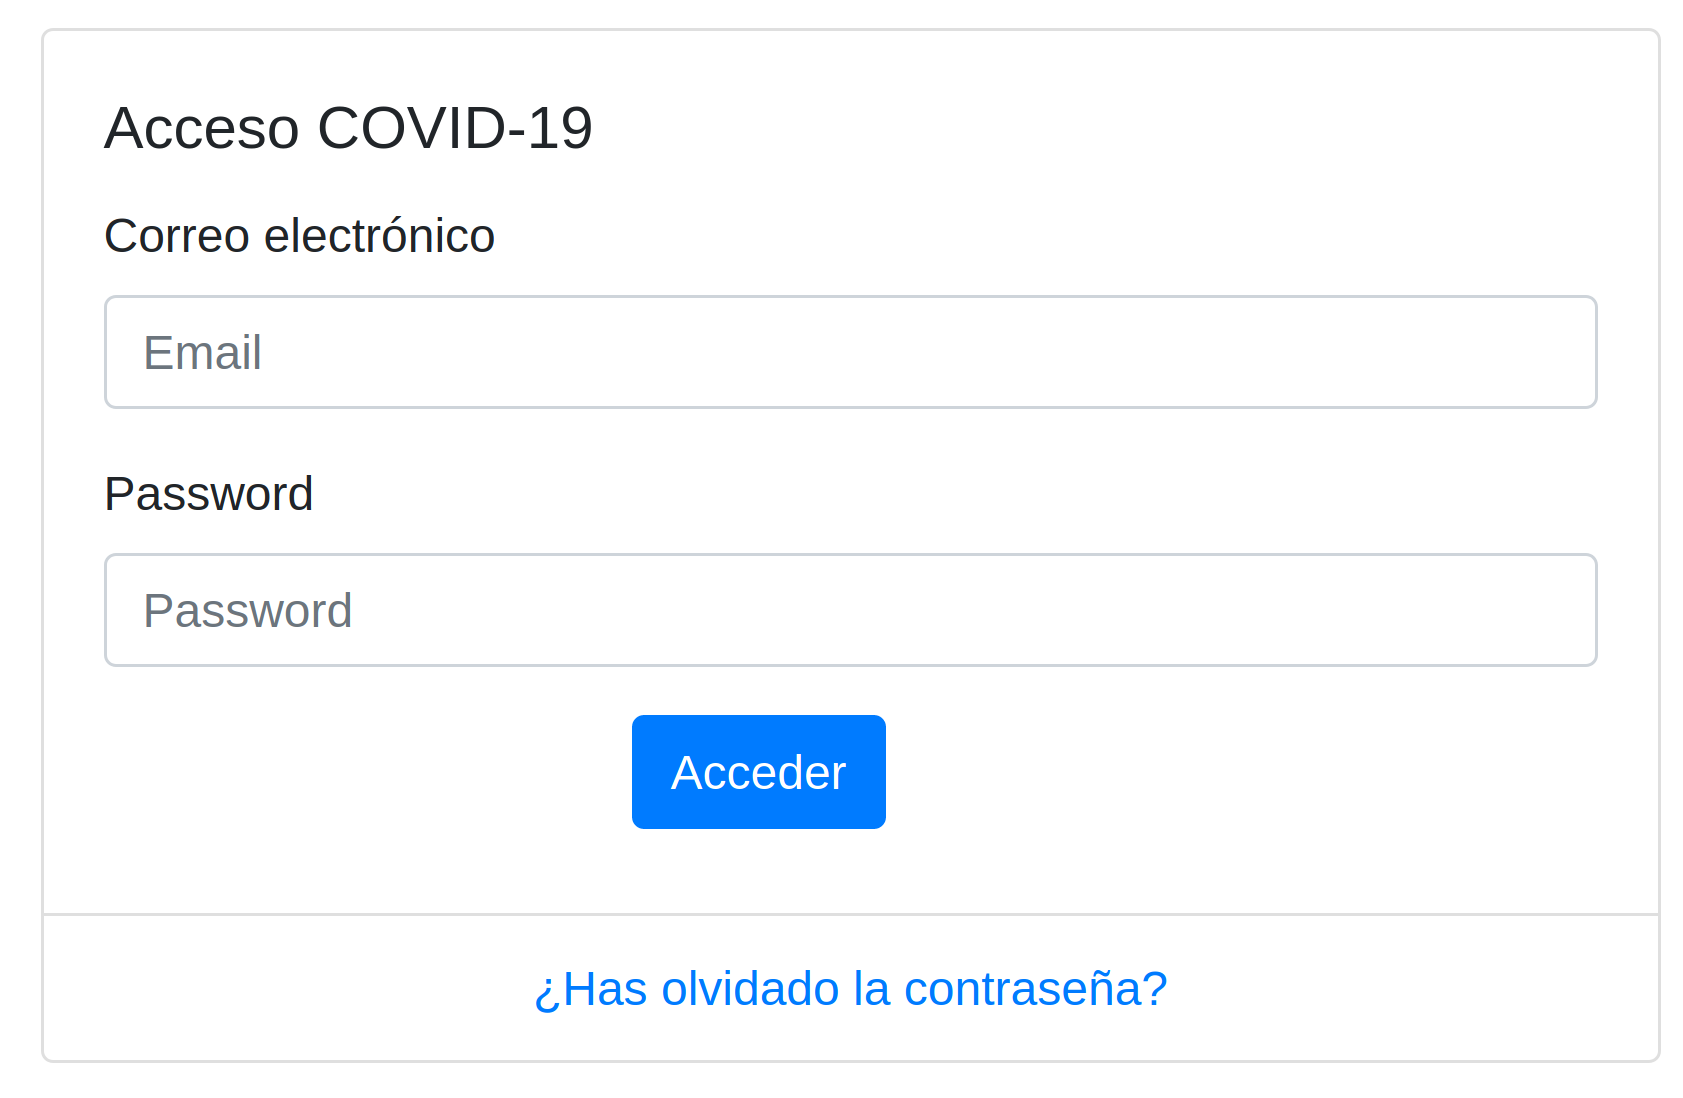
\includegraphics[scale=0.6]{Figs/Fig1.png}
\caption{Página de acceso a la plataforma}
\label{Fig1}
\end{figure}


\section{Rol CENTRO DE SALUD}    

El acceso con un correo identificado con el rol \textit{CENTRO DE SALUD}, nos permitirá la realización de una serie de tareas específicas de dicho rol. En particular:

\begin{enumerate}
    \item Nueva muestra
    \item Búsqueda de muestras
    \item Nuevo lote
    \item Búsqueda de lotes
\end{enumerate}

tal y como aparece en el menú desplegable.

\begin{figure}[h]
\centering
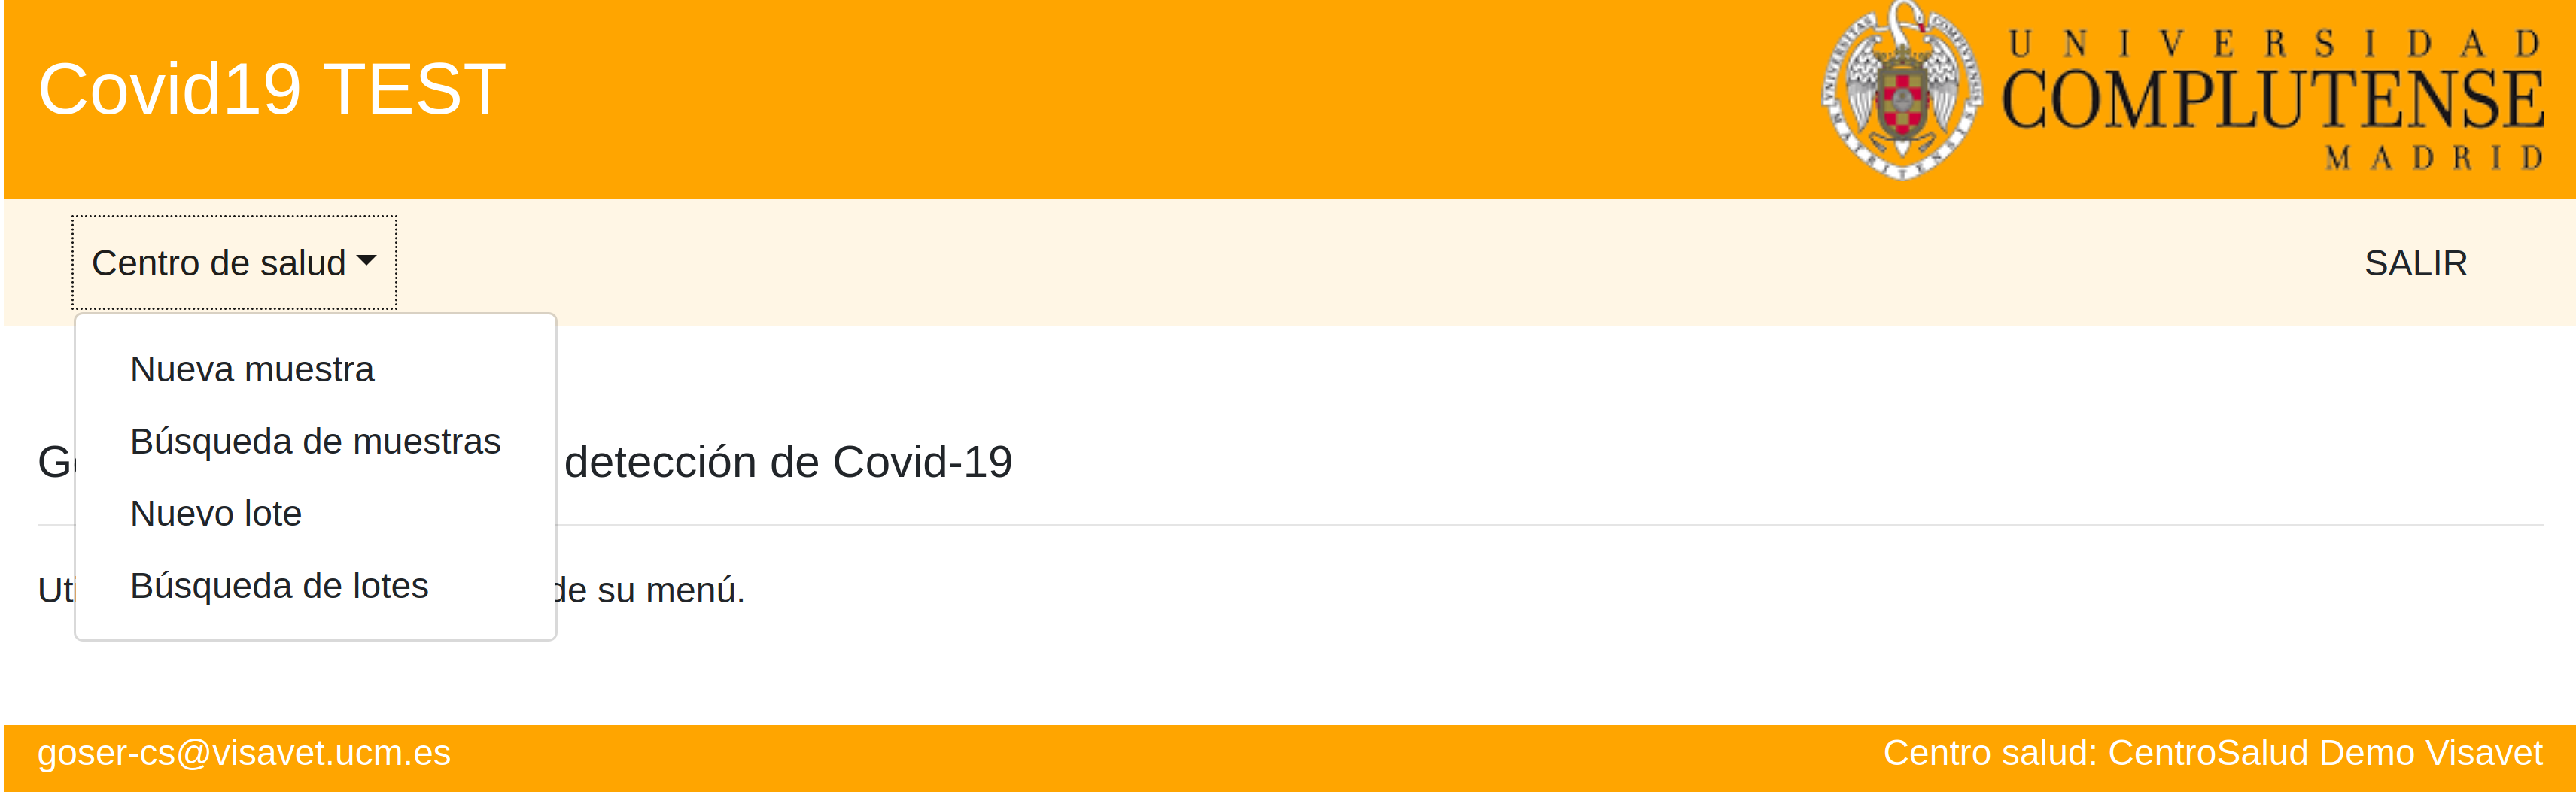
\includegraphics[scale=0.6]{Figs/Fig2.png}
\caption{Tareas del rol CENTRO DE SALUD}
\label{Fig2}
\end{figure}

\medskip
\begin{tcolorbox}[colback=blue!3!white,colframe=blue(ryb)!50!black,title=\textbf{Tip}]

Es posible saber en todo momento nuestro rol dentro del sistema gracias al mensaje del final de pantalla donde se muestra la información del acceso.

\end{tcolorbox}

\subsection{Nueva Muestra}

Esta pantalla permitirá dar de alta en el sistema una nueva muestra que debe ser enviada para análisis PCR. Además de los datos personales del paciente y su número de historia clínica (NHC), se recogerá la siguiente información:

\begin{itemize}
    \item Recoger datos para notificar: El centro de salud se encargará de la notificación de resultados al paciente.
    \item Notificar paciente automáticamente: El paciente recibirá un email con los resultados de la PCR.
    \item Avisar al paciente por sms: El paciente será notificado de los resultados mediante un SMS.
    
\end{itemize}

Así mismo, esta pantalla permite la identificación precisa de la muestra, cuyos datos serán verificados a lo largo del proceso de análisis para realizar su seguimiento:

\begin{itemize}
    \item Etiqueta: individual y específica de la muestra.
    \item Tipo de muestra: identificando cómo se ha obtenido.
    \item Fecha: de obtención de la muestra.
    \item Lote: al cual es asignado la muestra y que posteriormente será enviado a laboratorio.
\end{itemize}

\begin{figure}[h]
\centering
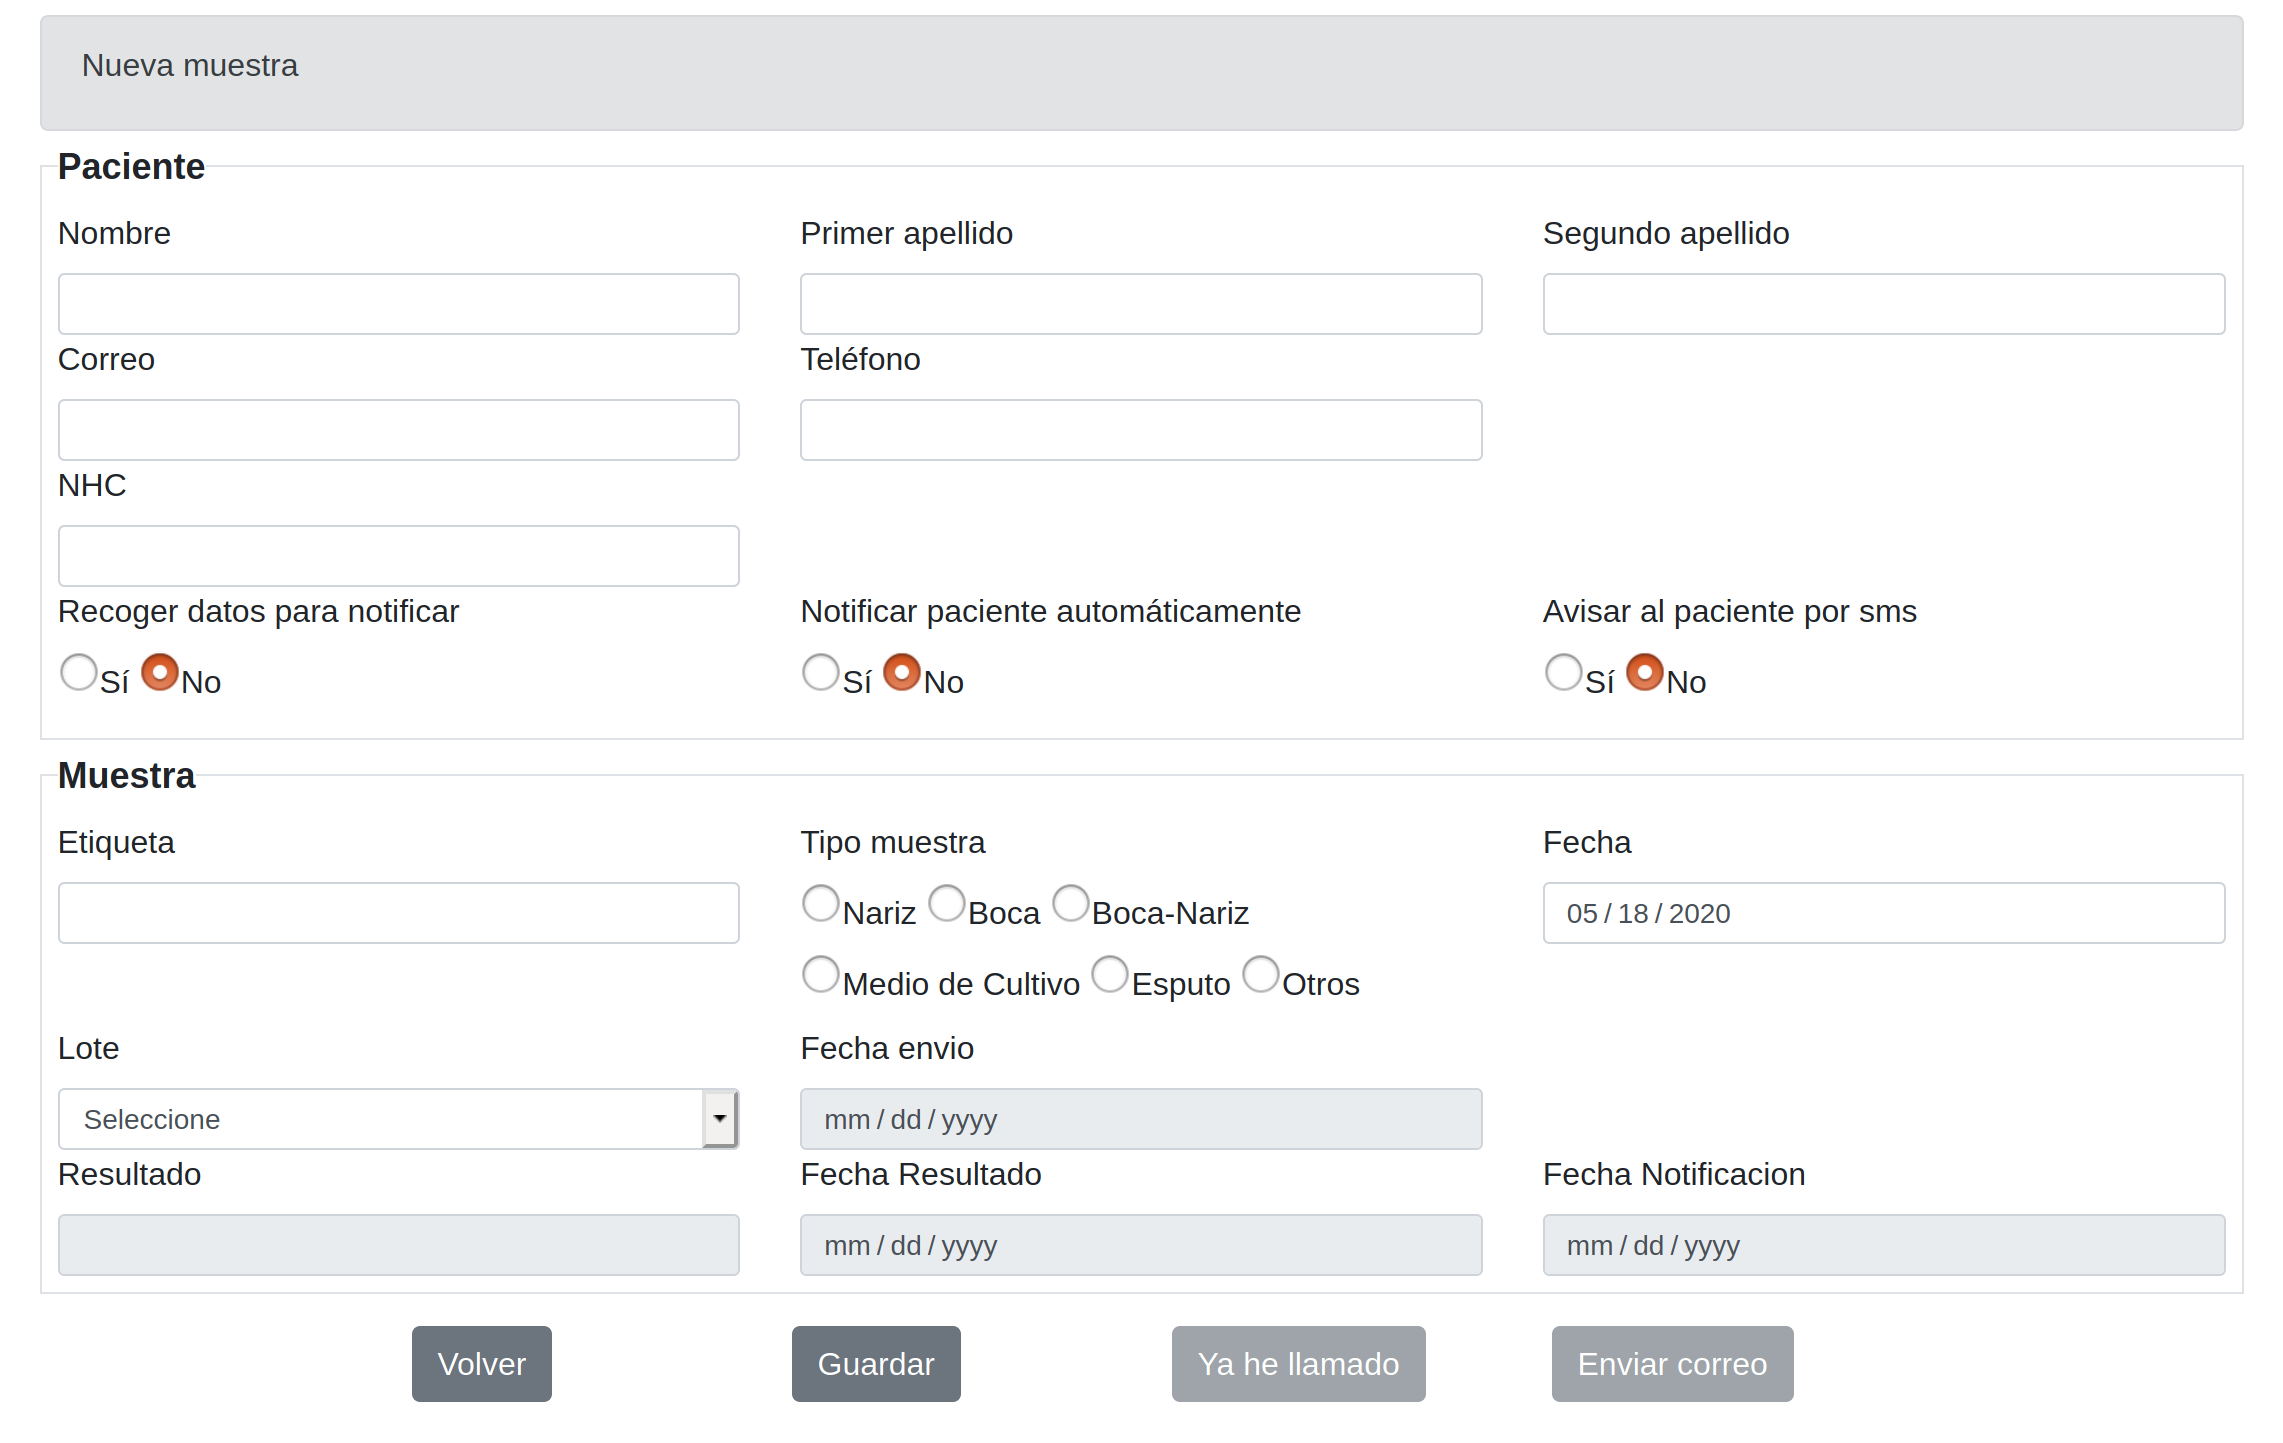
\includegraphics[scale=0.6]{Figs/Fig3.png}
\caption{Nueva Muestra}
\label{Fig3}
\end{figure}

Una vez complimentados los campos, deberemos grabar la muestra haciendo click en el botón GUARDAR.

El resto de campos de esta pantalla estarán disponibles una vez la muestra haya sido procesada, indicándonos tanto el resultado del análisis, como si el paciente ha sino notificado o no del resultado.

\subsection{Búsqueda de muestras}

Desde esta pantalla se podrá hacer una búsqueda de todas las muestras dadas de alta por el centro de salud. La búsqueda puede hacerse por cualquier campo conocido del paciente: nombre, apellido, NHC, correo; así como por datos de la muestra: estado, resultado, o fecha de envío a laboratorio.

El resultado de la búsqueda será un listado de muestras que cumplen los parámetros. Además, entre las opciones posibles tendremos la de editar o borrar los datos de la muestra (siempre que ésta no haya sido enviada aún a laboratorio).

\begin{figure}[h]
\centering
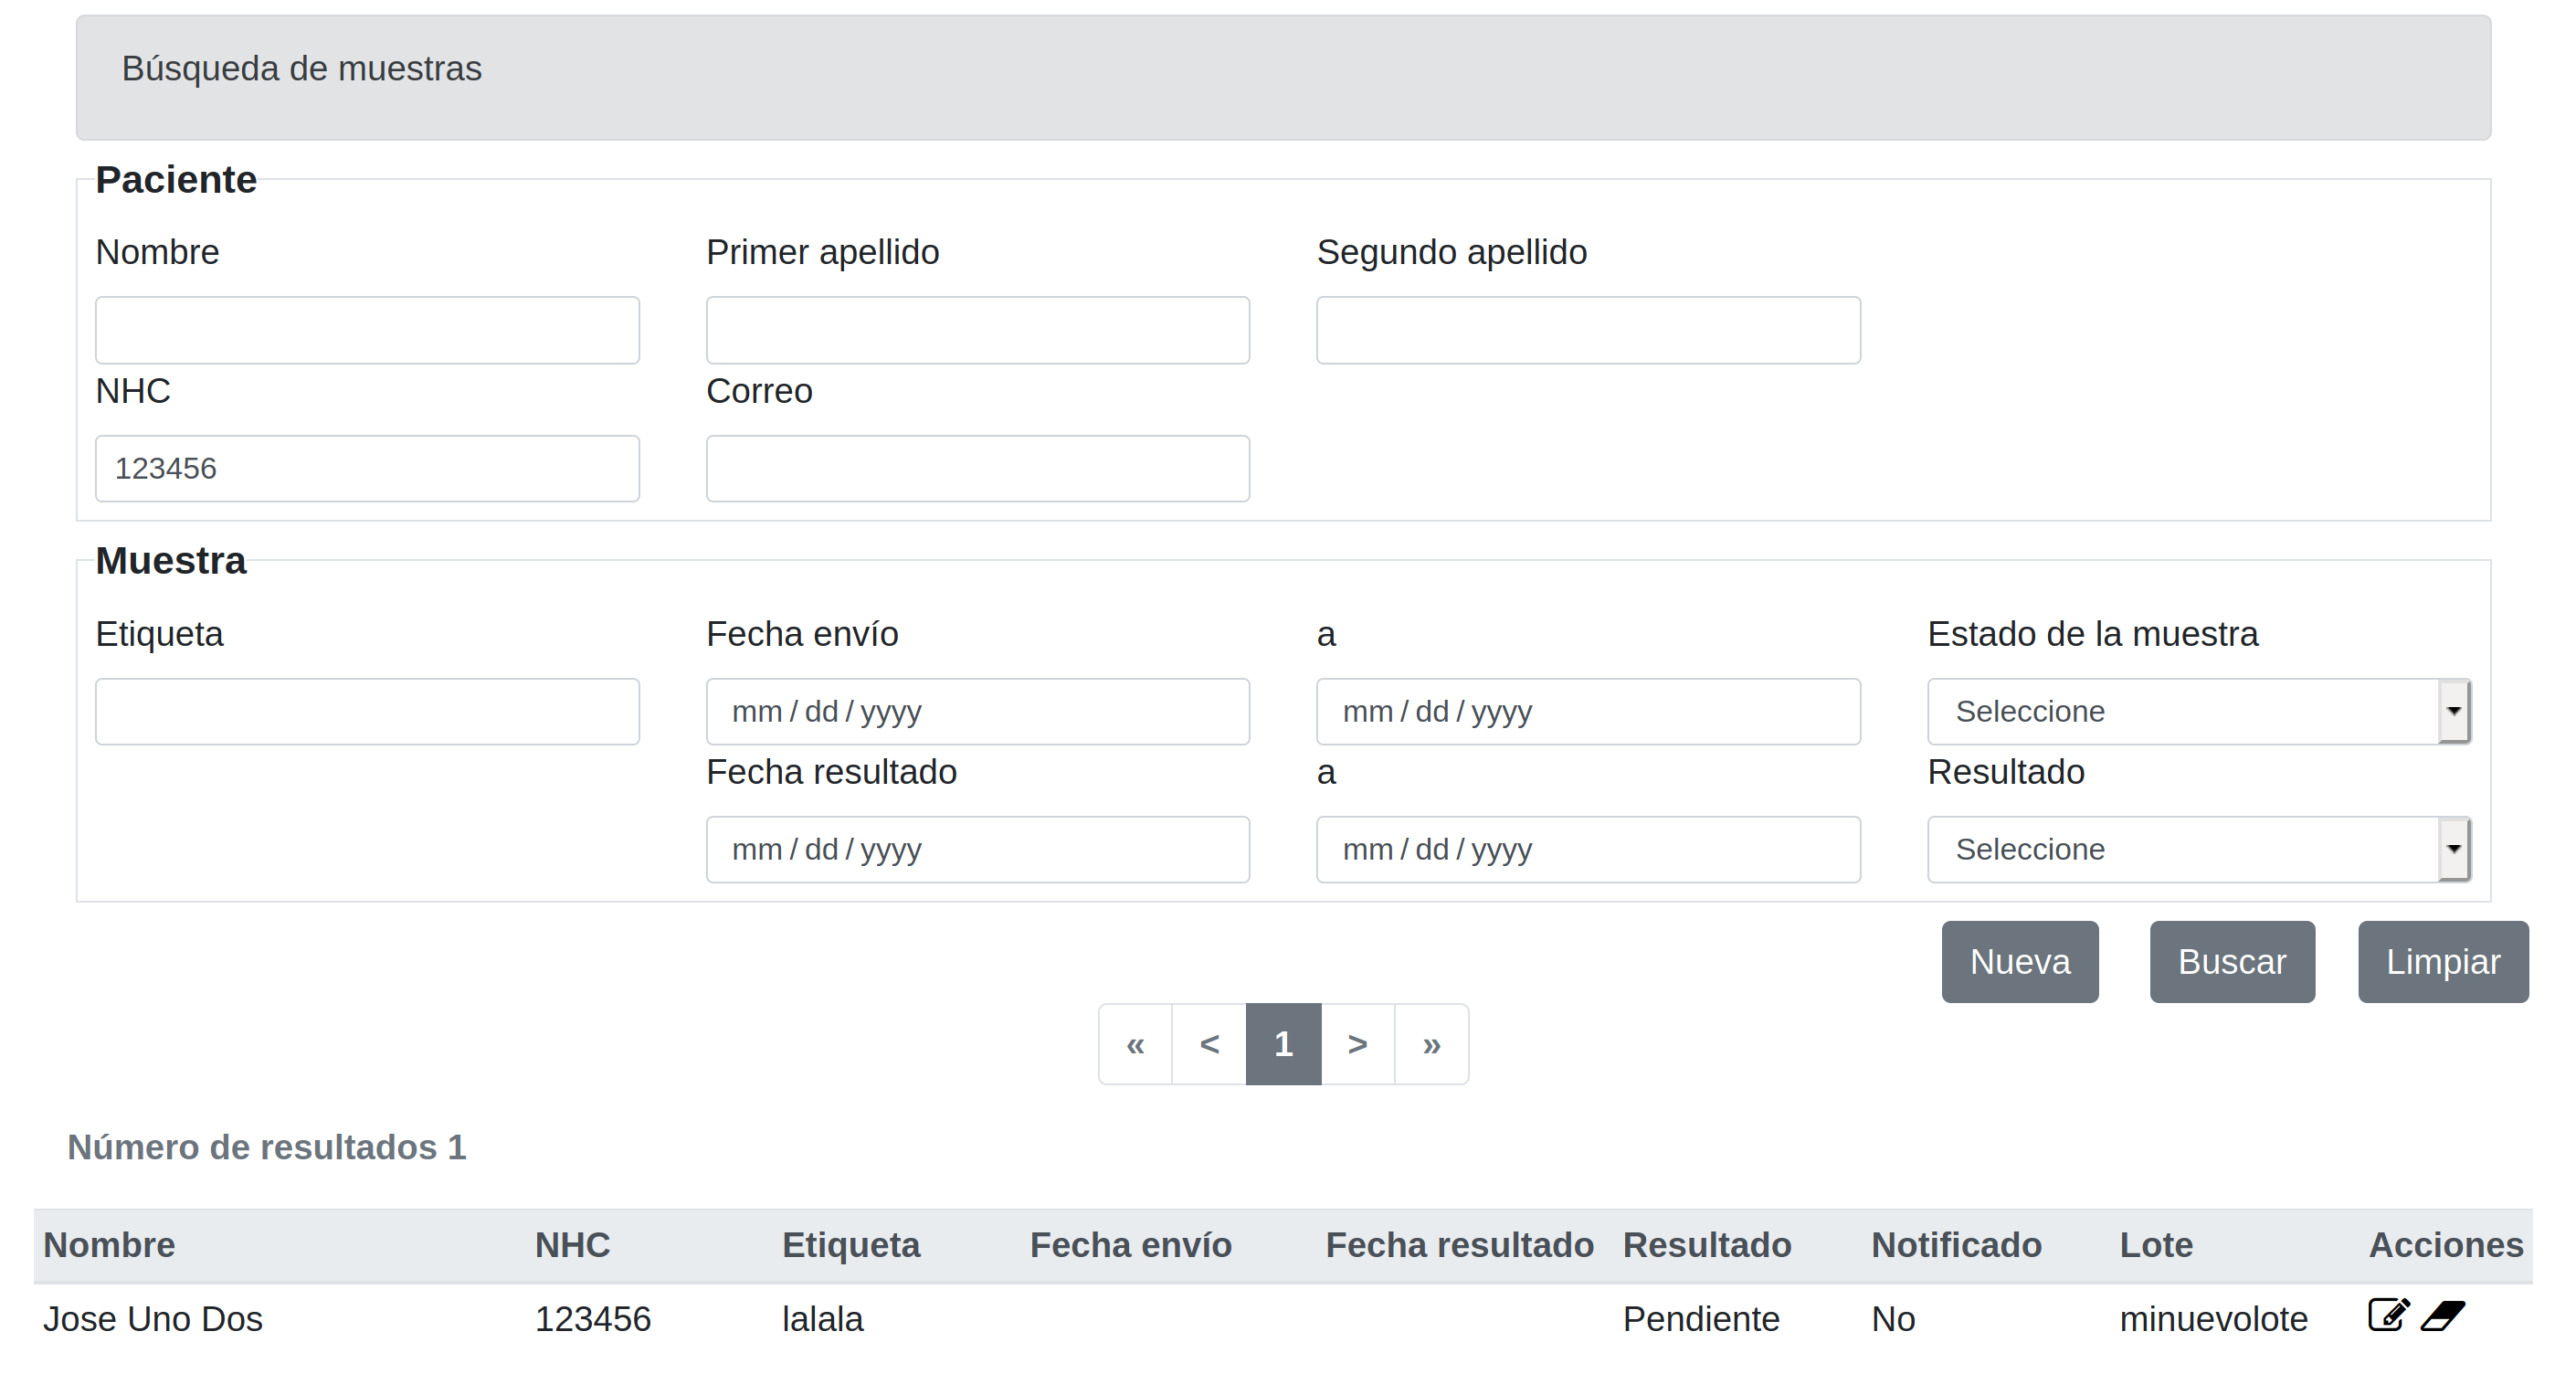
\includegraphics[scale=0.6]{Figs/Fig4.png}
\caption{Búsqueda de muestras}
\label{Fig4}
\end{figure}

\subsection{Nuevo lote}

Desde el rol CENTRO DE SALUD tenemos también la posibilidad de dar de alta un nuevo lote, siendo éste un conjunto de muestras que deberán ser enviadas todas juntas a laboratorio.

El lote vendrá identificado por un \emph{código} a elegir por el centro de salud, y deberá especificarse la \emph{capacidad} del mismo (número de muestras que puede contener dicho lote). Así mismo, deberemos indicar el \emph{laboratorio} que procesará dicho lote y donde debemos hacer llegar las muestras. 

\medskip
\begin{tcolorbox}[colback=blue!3!white,colframe=blue(ryb)!50!black,title=\textbf{Tip}]

El laboratorio, una vez recibido un lote para su procesamiento, verificará que está asignado a él. En caso contrario, no realizará el procesamiento de las muestras.

\end{tcolorbox}

\subsection{Búsqueda de lotes}

Esta opción del menú nos permite acceder a la información sobre los lotes existentes en el centro de salud. Mediante una búsqueda por parámetros (código del lote, estado, o fecha de envío, podremos acceder al listado de lotes.

\medskip
\begin{tcolorbox}[colback=blue!3!white,colframe=blue(ryb)!50!black,title=\textbf{Tip}]

Si dejamos en blanco todos los parámetros de búsqueda y hacemos click en el botón BUSCAR, podremos desplegar un listado completo de lotes generados por el centro de salud.

\end{tcolorbox}

\begin{figure}[h]
\centering
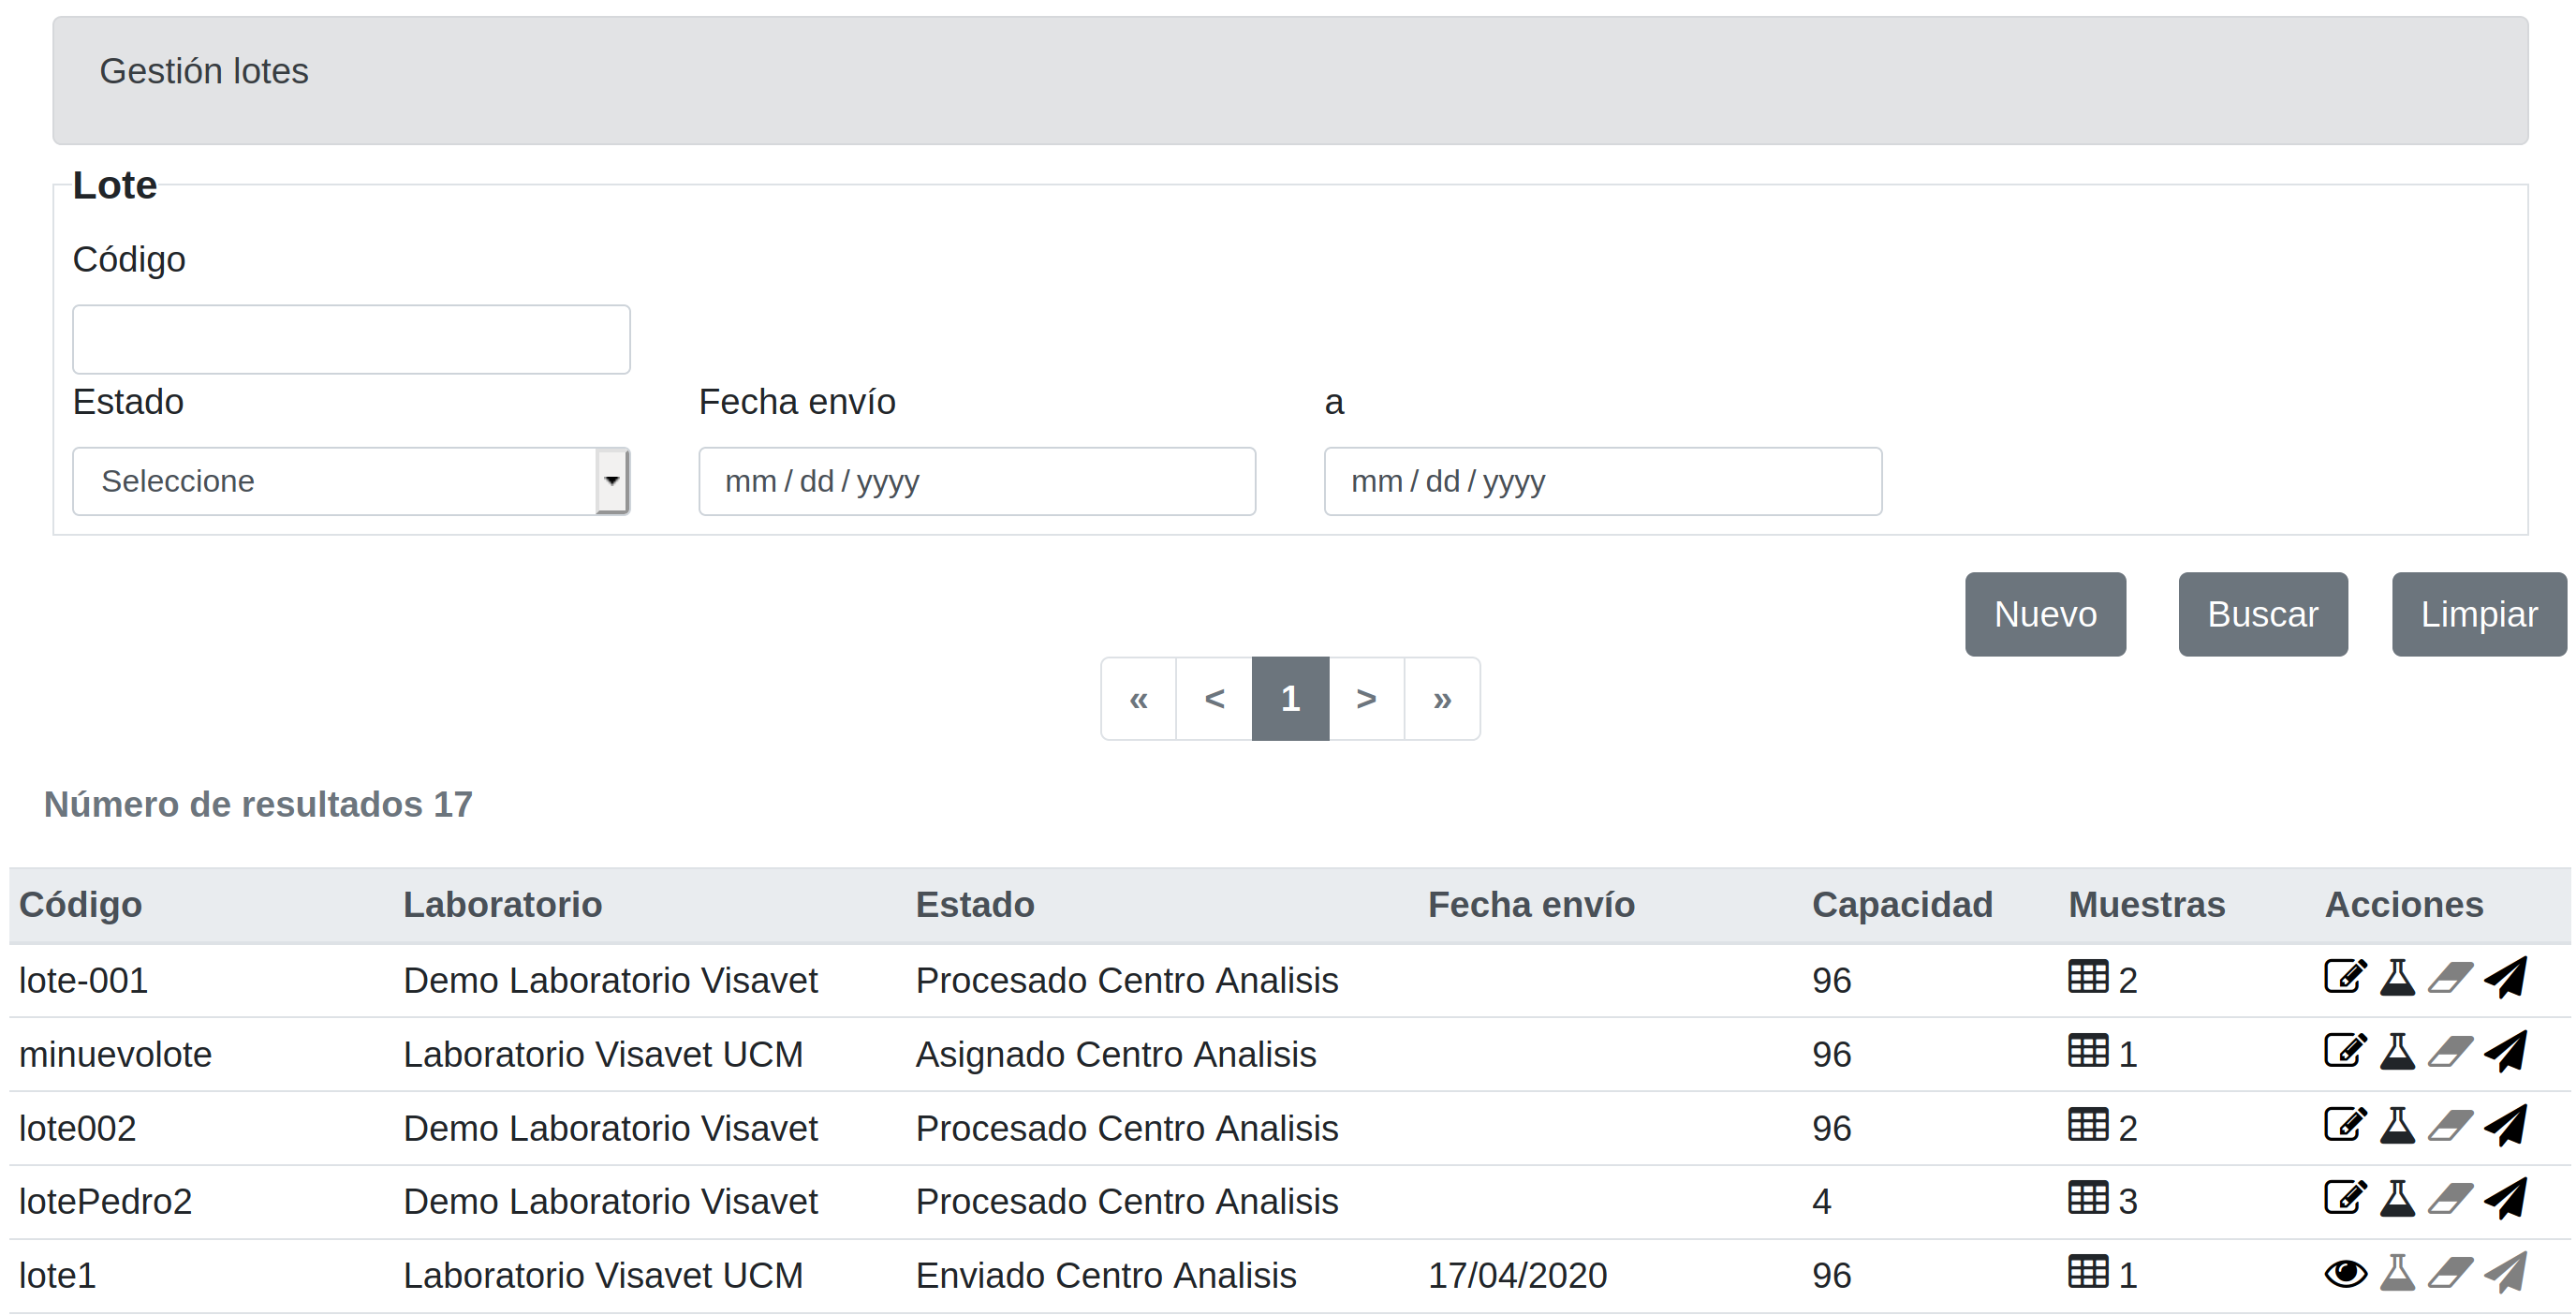
\includegraphics[scale=0.6]{Figs/Fig5.png}
\caption{Búsqueda de lotes}
\label{Fig5}
\end{figure}

Dentro del listado de muestras, podremos acceder a diversas acciones sobre el lote en cuestión, como:

\begin{itemize}
    \item \emph{ver las muestras del lote}
    
\begin{figure}[h]
\centering
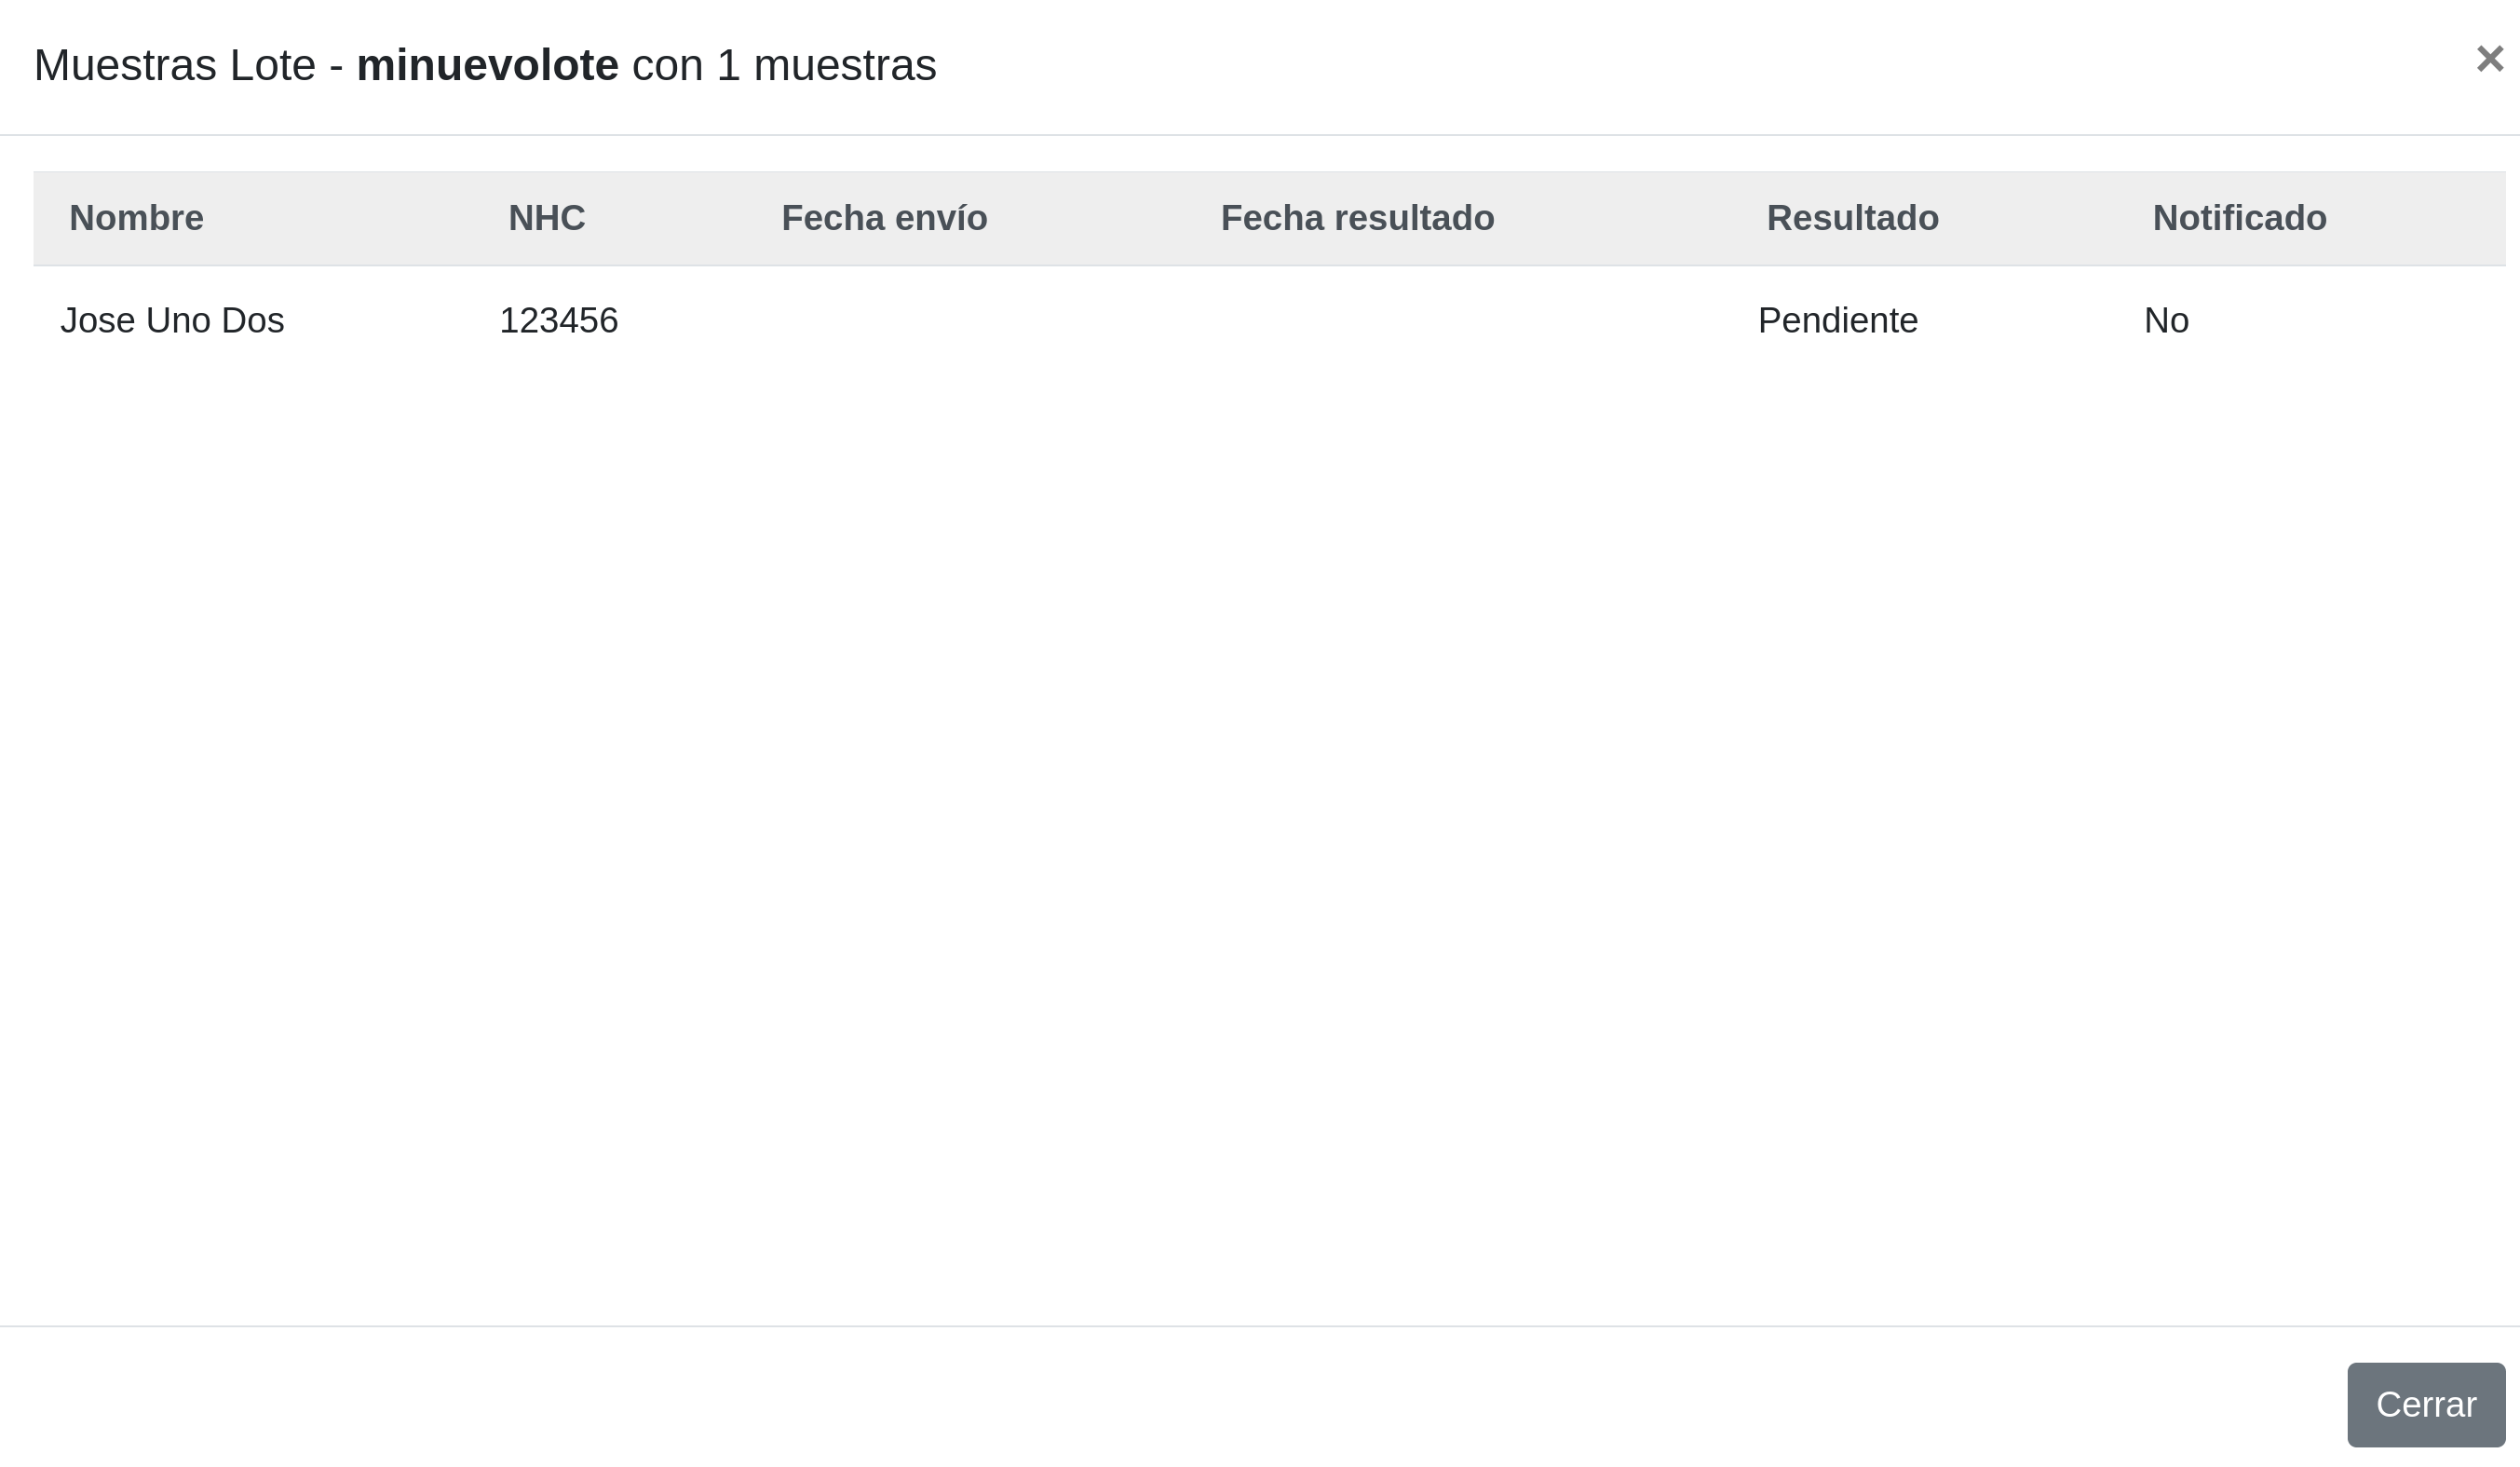
\includegraphics[scale=0.6]{Figs/Fig6.png}
\caption{Ver muestras en lote}
\label{Fig6}
\end{figure}

    
    \item \emph{modificar la información del lote (antes de que éste haya sido enviado al laboratorio)}
    
\begin{figure}[h]
\centering
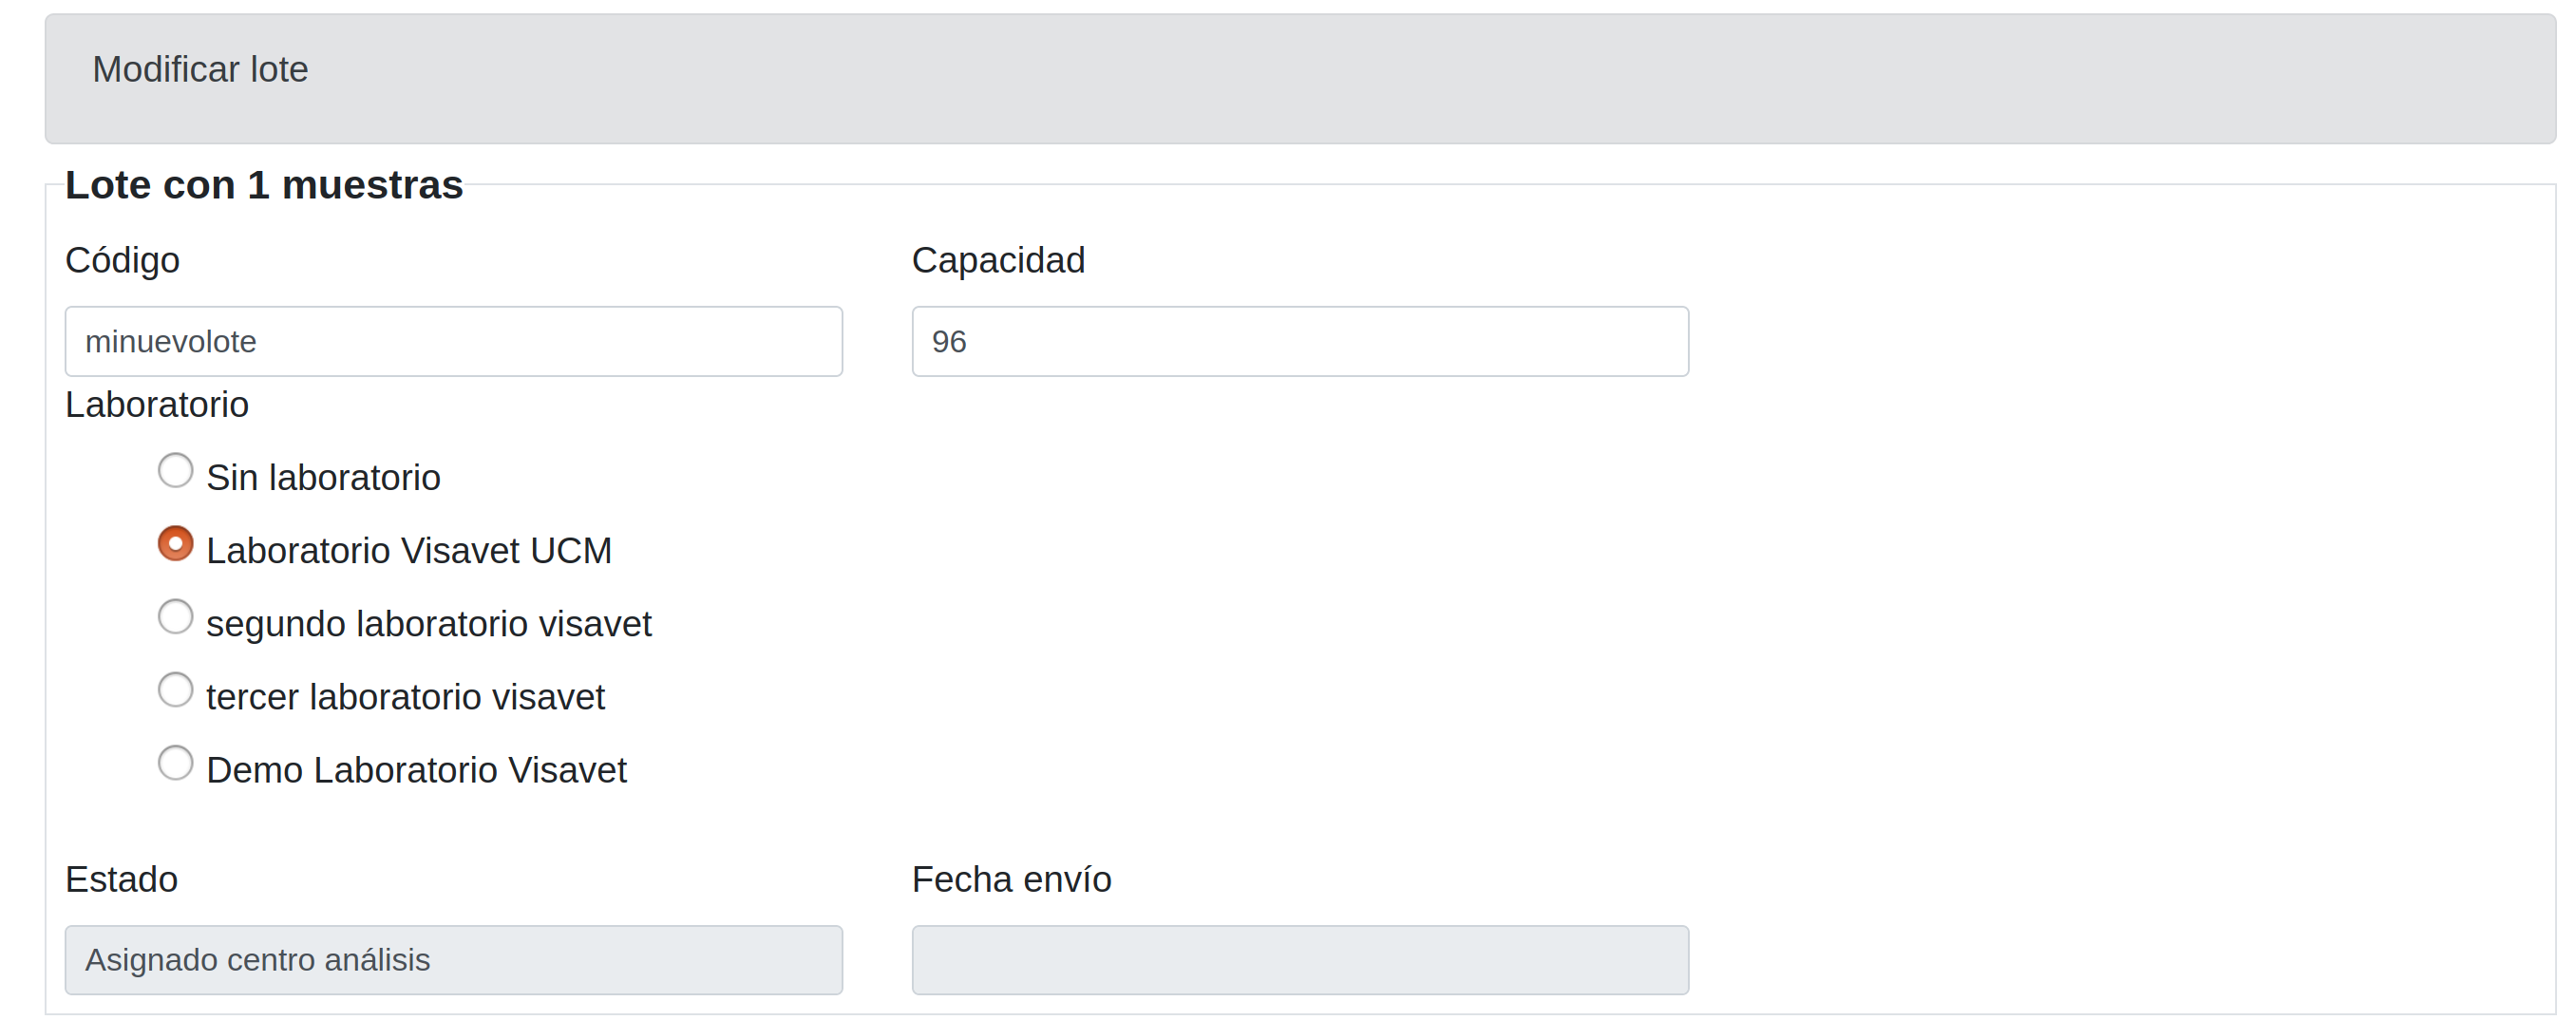
\includegraphics[scale=0.6]{Figs/Fig7.png}
\caption{Modificar información del lote}
\label{Fig7}
\end{figure}

    
    \item \emph{cambiar el laboratorio asignado para el procesamiento del lote}
    
\begin{figure}[h]
\centering
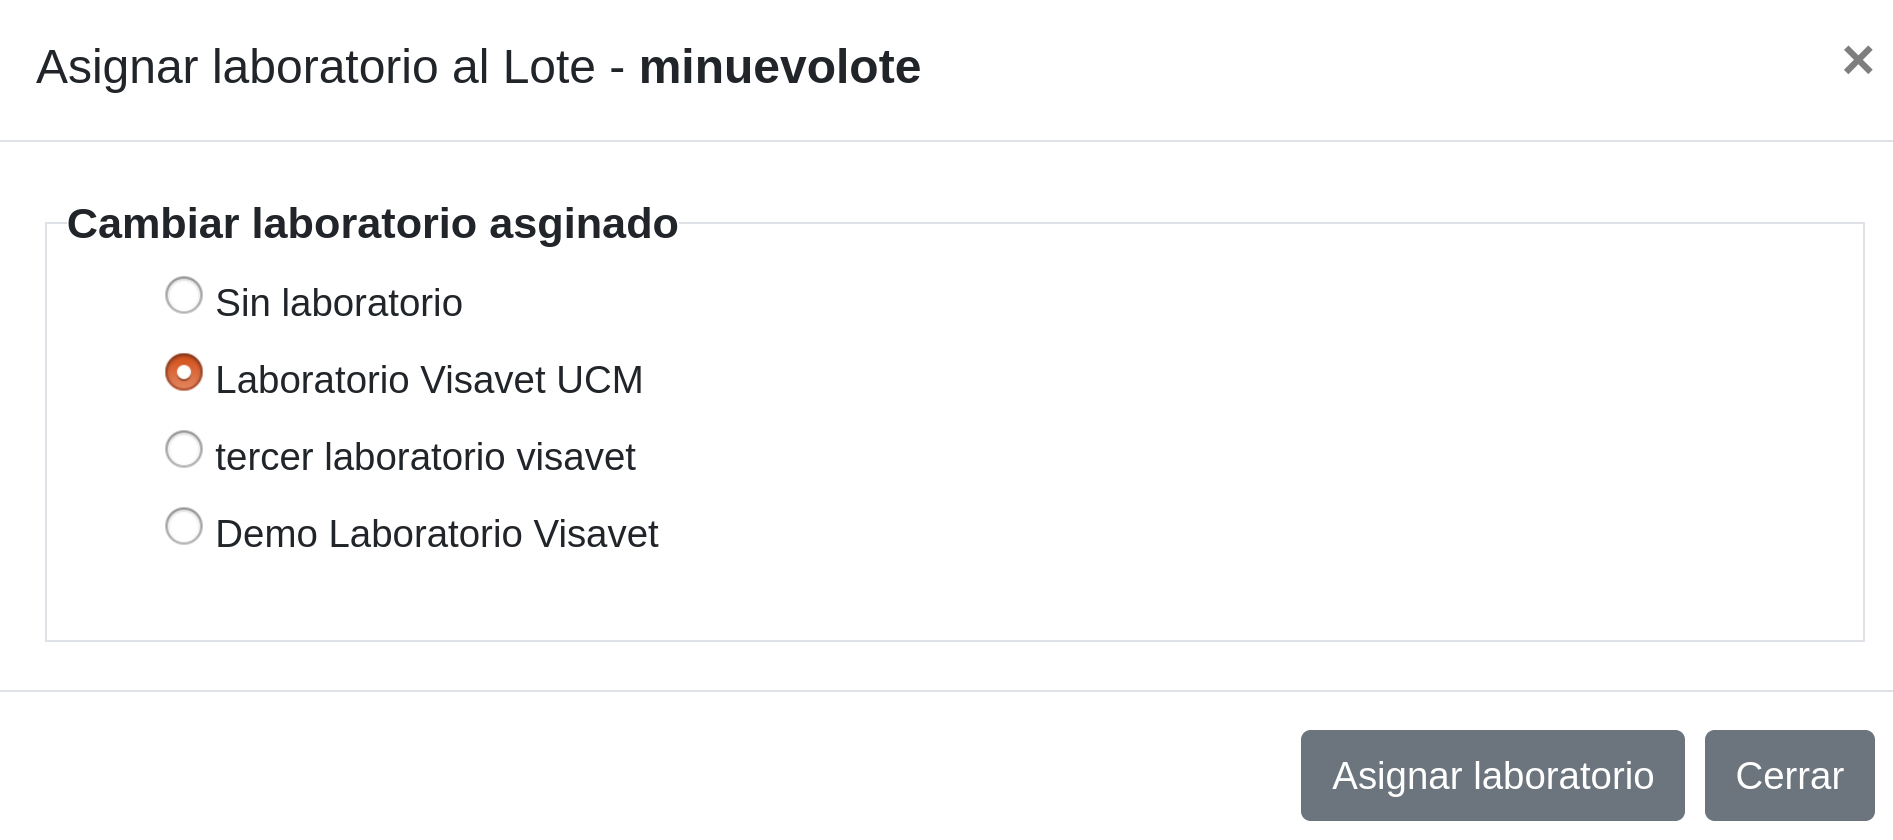
\includegraphics[scale=0.6]{Figs/Fig8.png}
\caption{Cambiar laboratorio asignado al lote}
\label{Fig8}
\end{figure}
    
    
    \item \emph{enviar el lote al laboratorio asignado para su procesamiento}
    
\begin{figure}[h]
\centering
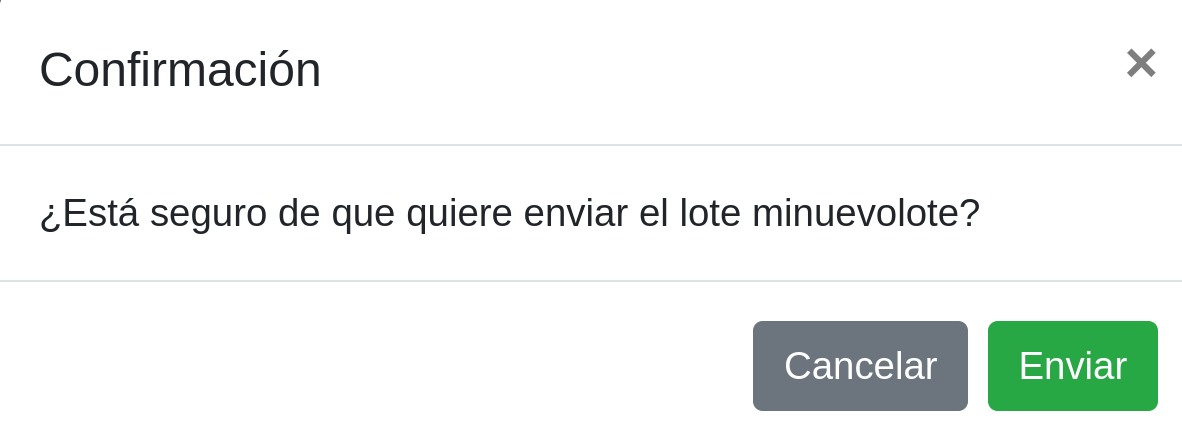
\includegraphics[scale=0.6]{Figs/Fig9.png}
\caption{Enviar lote al laboratorio}
\label{Fig9}
\end{figure}

    
\end{itemize}

\medskip
\begin{tcolorbox}[colback=blue!3!white,colframe=blue(ryb)!50!black,title=\textbf{Tip}]

Una vez enviado el lote al laboratorio desde la aplicación informática, es indispensable hacer el envío físico de las muestras a través del servicio de mensajería dispuesto al efecto.

\end{tcolorbox}

\section{Rol RECEPCIÓN LABORATORIO}

El acceso con un corredo indentificado con el RECEPCIÓN LABORATORIO nos permitirá la confirmación de la recepción de lotes.

\begin{figure}[h]
\centering
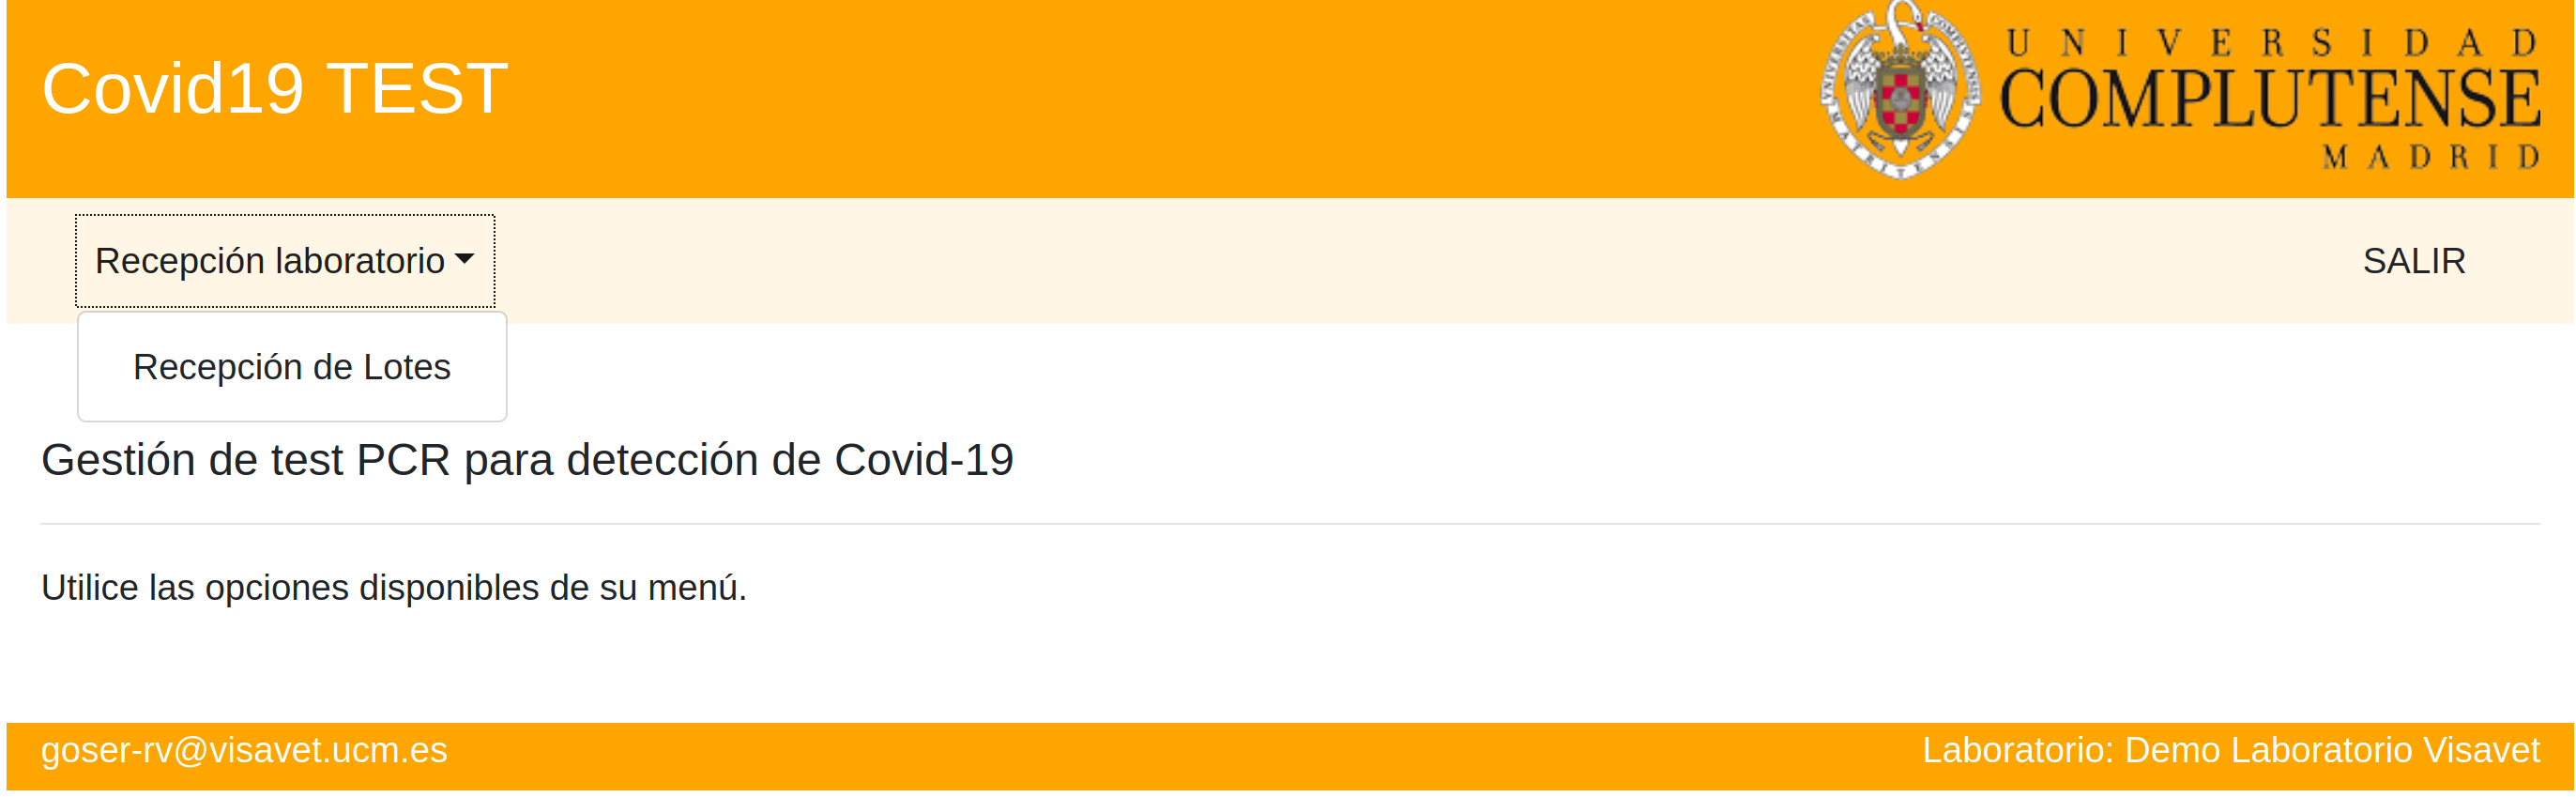
\includegraphics[scale=0.6]{Figs/Fig10.png}
\caption{Tareas del rol RECEPCIÓN LABORATORIO}
\label{Fig10}
\end{figure}

\medskip
\begin{tcolorbox}[colback=blue!3!white,colframe=blue(ryb)!50!black,title=\textbf{Tip}]

Es posible saber en todo momento nuestro rol dentro del sistema gracias al mensaje del final de pantalla donde se muestra la información del acceso..

\end{tcolorbox}

\subsection{Recepción de lotes}

La única tarea disponible dentro de este rol es la \emph{recepción de lotes}, que permite verificar que el laboratorio ha recibido físicamente los lotes de muestras asignados a él por el centro de salud.

Así, dentro de la pantalla de recepción de lotes, se podrá hacer una búsqueda de los lotes asignados al laboratorio por el centro de salud y que debieran haberse recibido. El laboratorio podrá realizar la búsqueda por: centro de procedencia, número de lote, estado, o fecha de análisis. Así, obtendremos un listado de los lotes de muestras que cumplen con las opciones de búsqueda.

\begin{figure}[h]
\centering
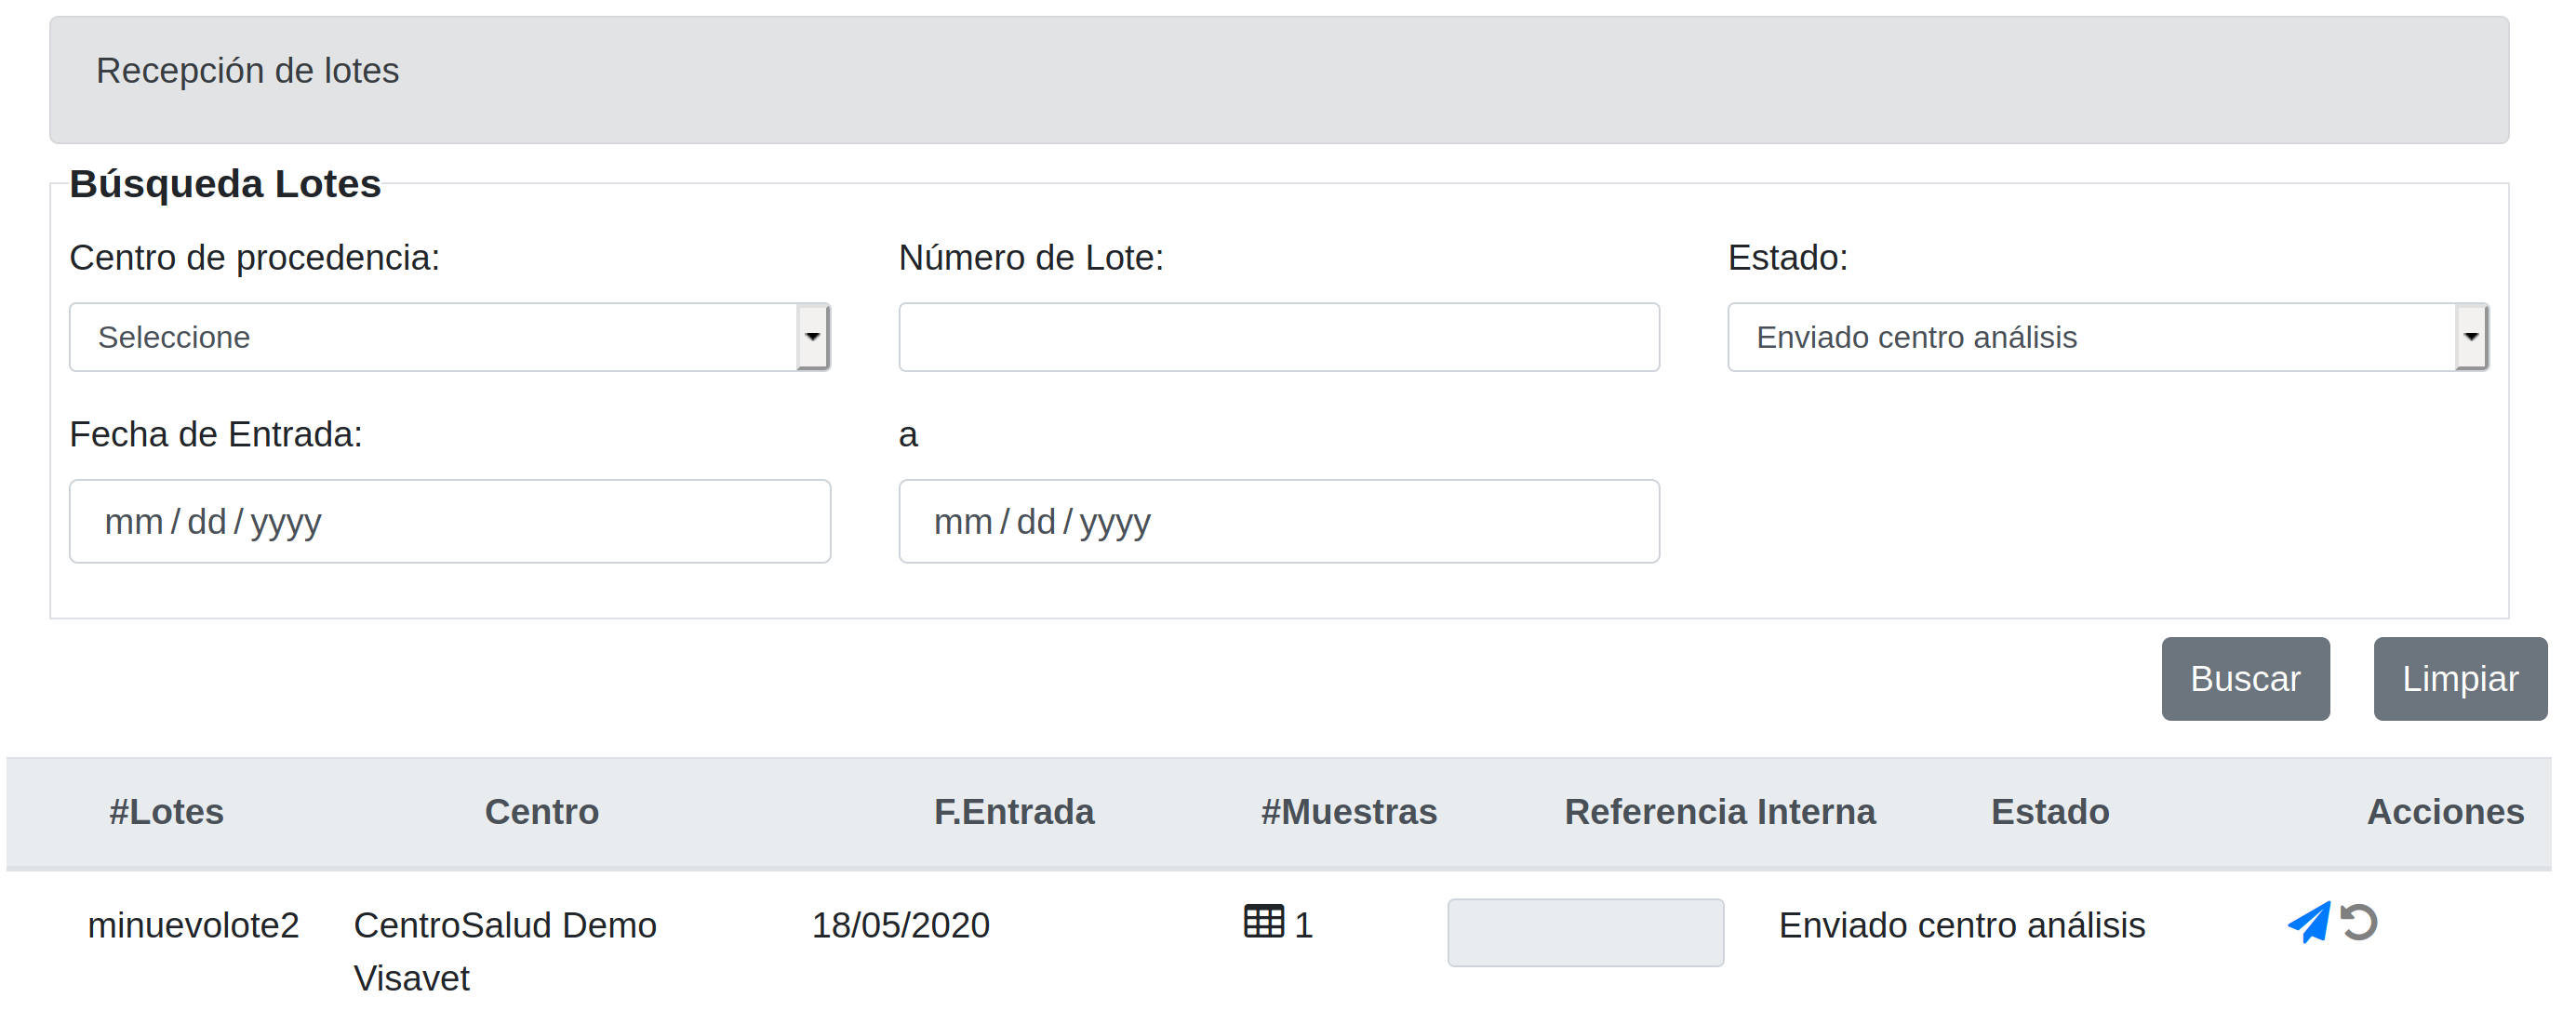
\includegraphics[scale=0.6]{Figs/Fig11.png}
\caption{Recepción de lotes}
\label{Fig11}
\end{figure}

\medskip
\begin{tcolorbox}[colback=blue!3!white,colframe=blue(ryb)!50!black,title=\textbf{Tip}]

Si dejamos en blanco todos los parámetros de búsqueda y hacemos click en el botón BUSCAR, podremos desplegar un listado completo de lotes asignados al laboratorio.

\end{tcolorbox}

Para cada uno de los lotes asignados al laboratorio, podremos verificar las muestras que contienen.

\begin{figure}[h]
\centering
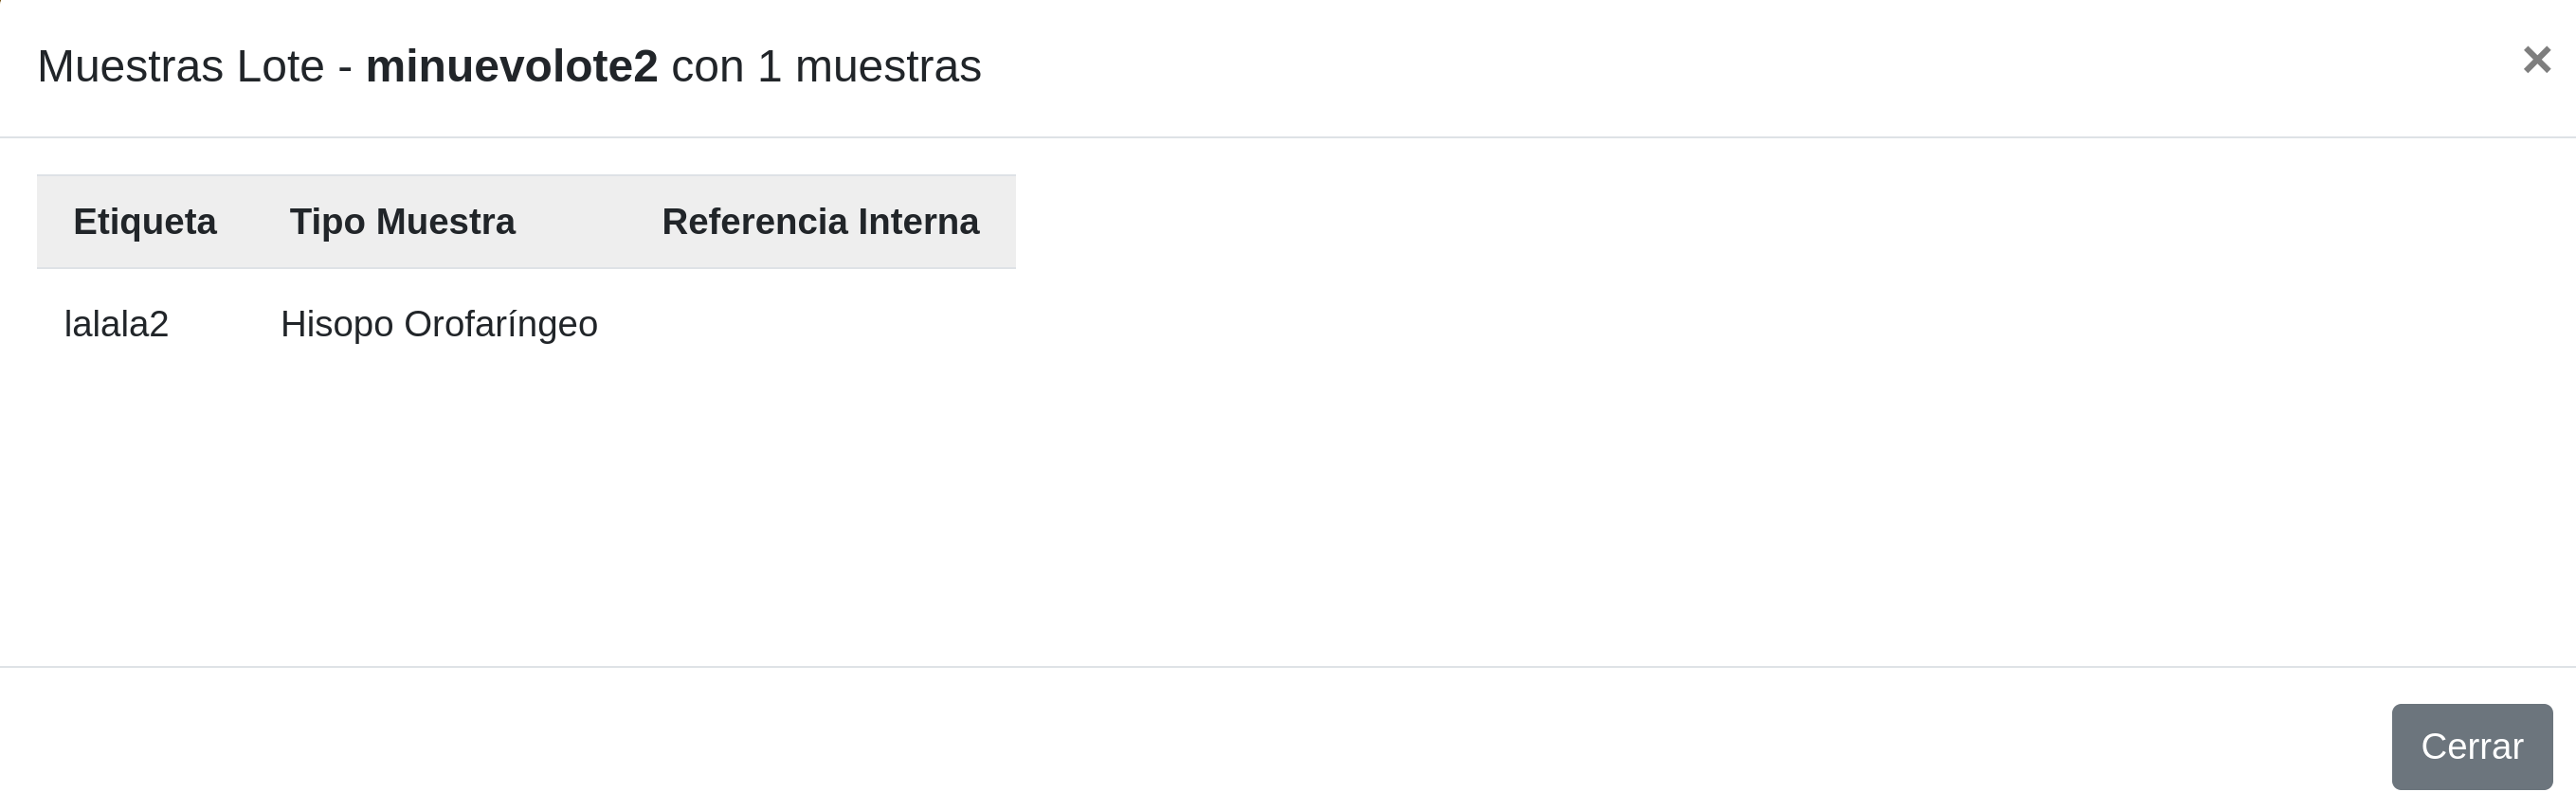
\includegraphics[scale=0.6]{Figs/Fig12.png}
\caption{Muestras contenidas en el lote}
\label{Fig12}
\end{figure}

Así como confirmar, o cancelar, la recepción del lote.

\begin{figure}[h]
\centering
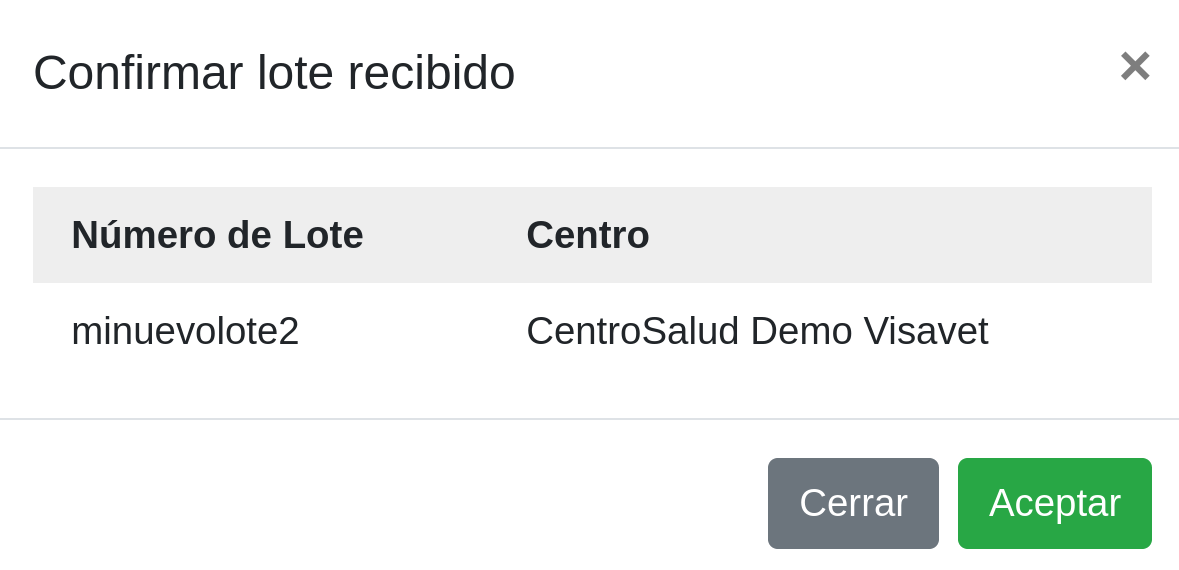
\includegraphics[scale=0.6]{Figs/Fig13.png}
\caption{Confirmar recepción del lote}
\label{Fig13}
\end{figure}

\medskip
\begin{tcolorbox}[colback=blue!3!white,colframe=blue(ryb)!50!black,title=\textbf{Tip}]

Verificar que el lote se encuentra en las instalaciones del laboratorio, que coinciden los datos de identificación del mismo, así como las muestras contenidas en él, antes de confirmar su recepción.

\end{tcolorbox}

\section{Rol TÉCNICO DE LABORATORIO}    

El acceso con un correo identificado con el rol \textit{TÉCNICO DE LABORATORIO}, nos permitirá la realización de una serie de tareas específicas de dicho rol. En particular:

\begin{enumerate}
    \item Asignar lotes a placas
    \item Gestionar placas
    \item Carga sin datos previos del centro de salud
\end{enumerate}

tal y como aparece en el menú desplegable.

\begin{figure}[h]
\centering
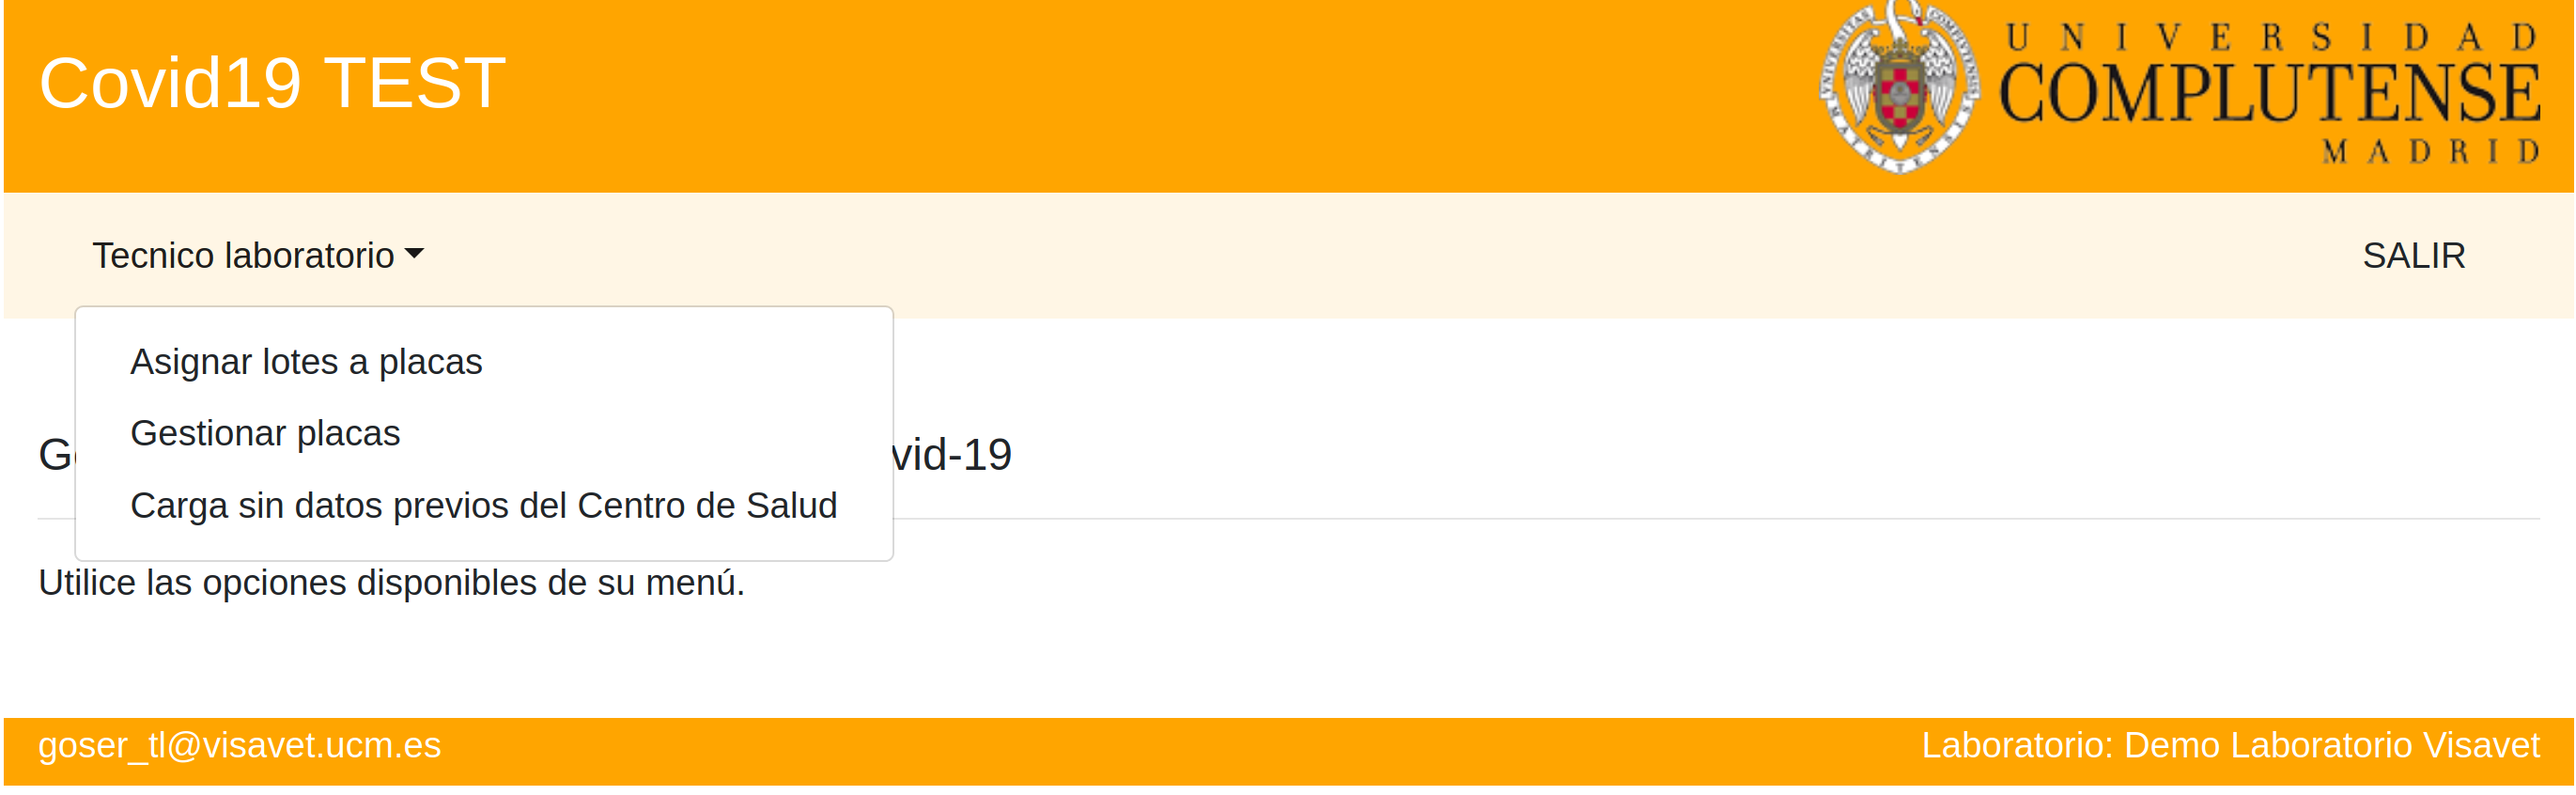
\includegraphics[scale=0.6]{Figs/Fig14.png}
\caption{Tareas del rol TÉCNICO DE LABORATORIO}
\label{Fig14}
\end{figure}

\medskip
\begin{tcolorbox}[colback=blue!3!white,colframe=blue(ryb)!50!black,title=\textbf{Tip}]

Es posible saber en todo momento nuestro rol dentro del sistema gracias al mensaje del final de pantalla donde se muestra la información del acceso.

\end{tcolorbox}

\subsection{Asignar lotes a placas}

La primera tarea que se puede hacer bajo el rol TÉCNICO DE LABORATORIO es asignar las muestras incluidas en los lotes recibidos en el laboratorio, a las placas de análisis que irán a PCR.

Para ello, se comenzará haciendo una búsqueda de los lotes recibidos haciendo uso de la herramientas de búsqueda (por centro de procedencia, número de lote, estado, o fecha de entrada). Dicha búsqueda proporcionará un listado de lotes disponibles en el laboratorio para su análisis.

\begin{figure}[h]
\centering
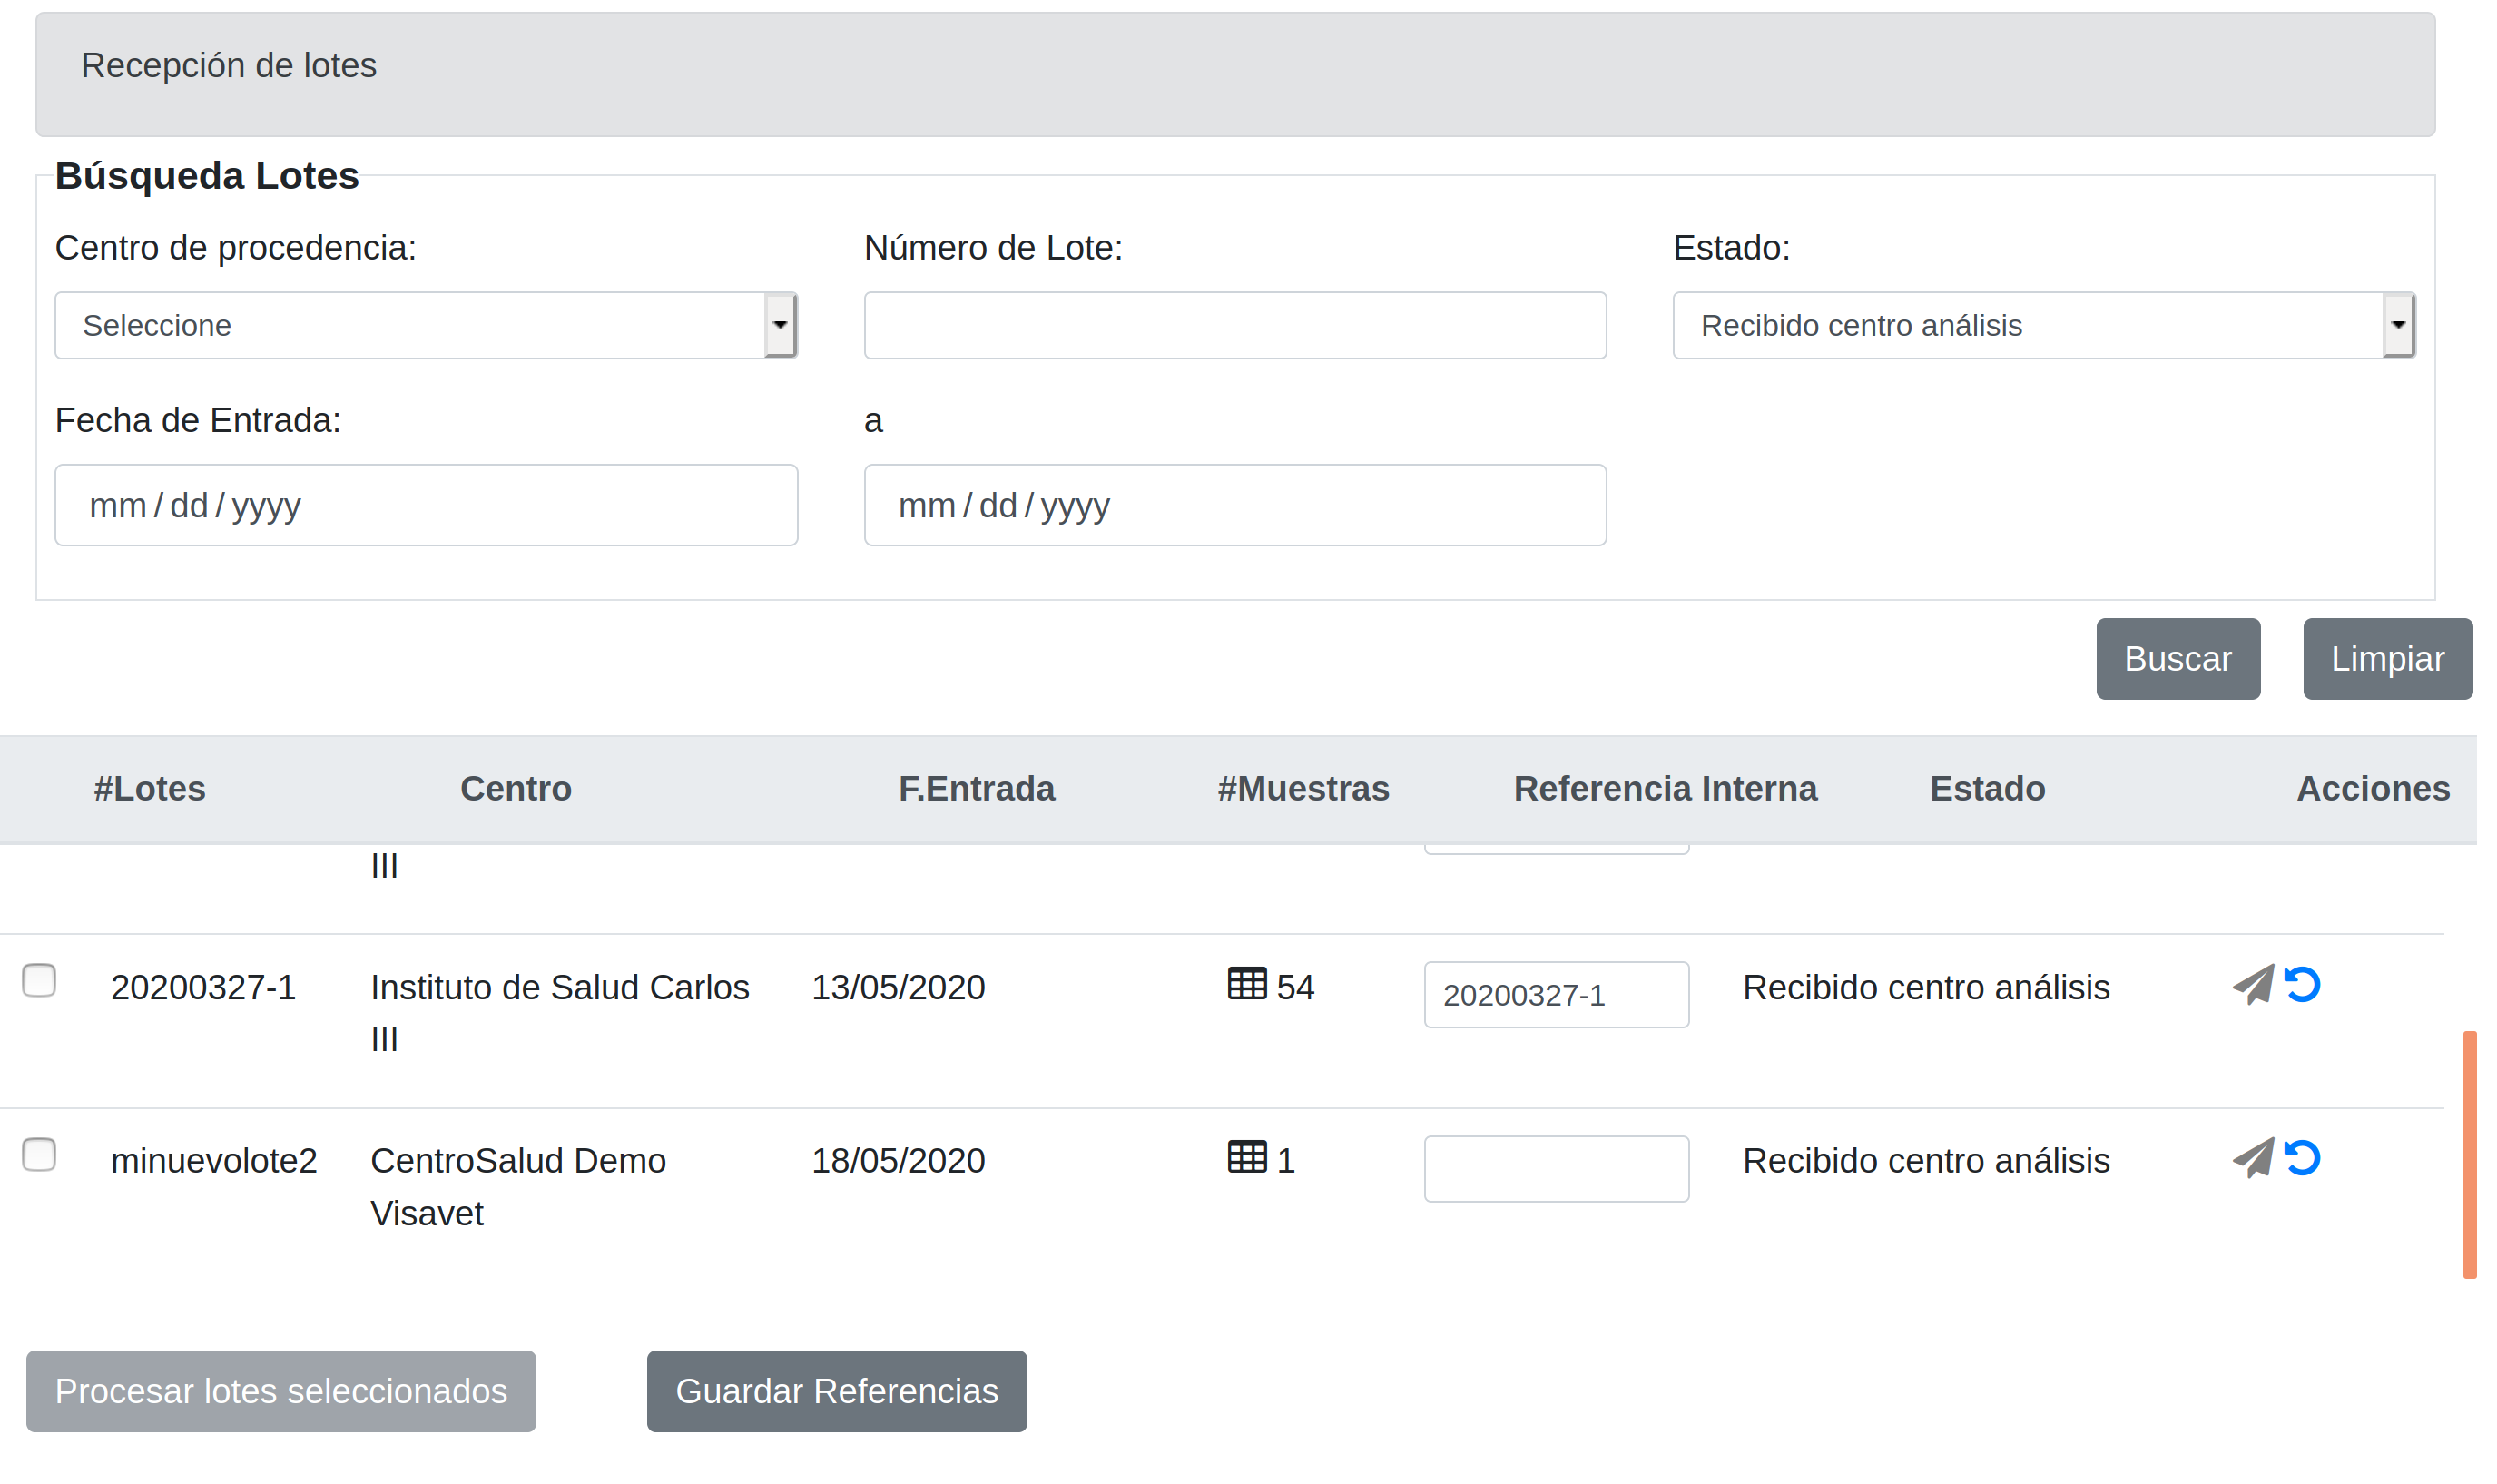
\includegraphics[width=0.7\textwidth]{Figs/Fig15.png}
\caption{Búsqueda de lotes}
\label{Fig15}
\end{figure}

\medskip
\begin{tcolorbox}[colback=blue!3!white,colframe=blue(ryb)!50!black,title=\textbf{Tip}]

Si dejamos en blanco todos los parámetros de búsqueda y hacemos click en el botón BUSCAR, podremos desplegar un listado completo de lotes generados por el centro de salud.

\end{tcolorbox}

Dentro del listado proporcionado por la búsqueda, podremos comprobar las muestras incluidas dentro de cada lote, que deberán coincider con las recibidas en el laboratorio.

\begin{figure}[h]
\centering
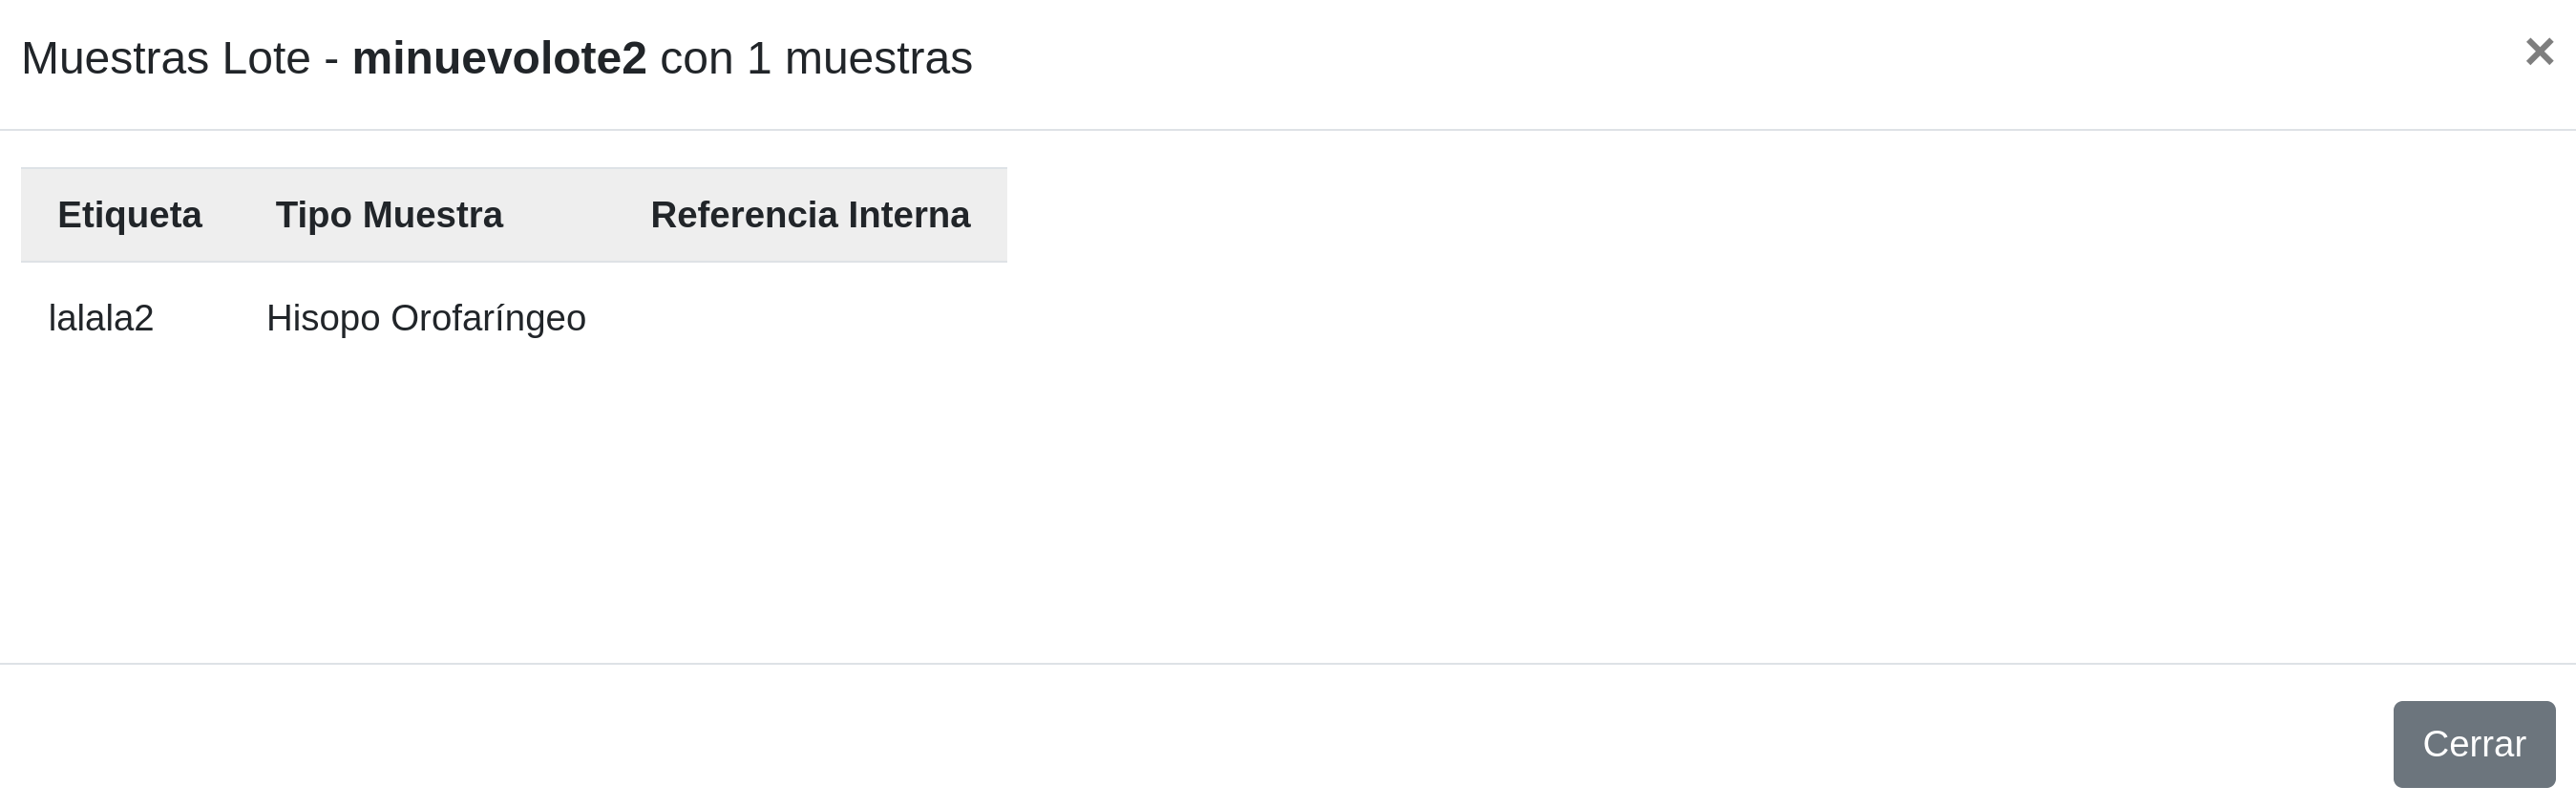
\includegraphics[width=0.6\textwidth]{Figs/Fig16.png}
\caption{Muestras incluidas en el lote}
\label{Fig16}
\end{figure}

También asignaremos una referencia interna al lote que permitirá su identificación dentro de la placa PCR.

\begin{figure}[h]
\centering

\includegraphics[width=0.6\textwidth]{Figs/Fig17.png}
\caption{Asignación de referencia interna a lote}
\label{Fig17}
\end{figure}

Finalmente, haciendo click sobre el botón PROCESAR LOTES SELECCIONADOS, podremos acceder a la opción de asignar una placa PCR al lote o lotes seleccionados.

\begin{figure}[h]
\centering
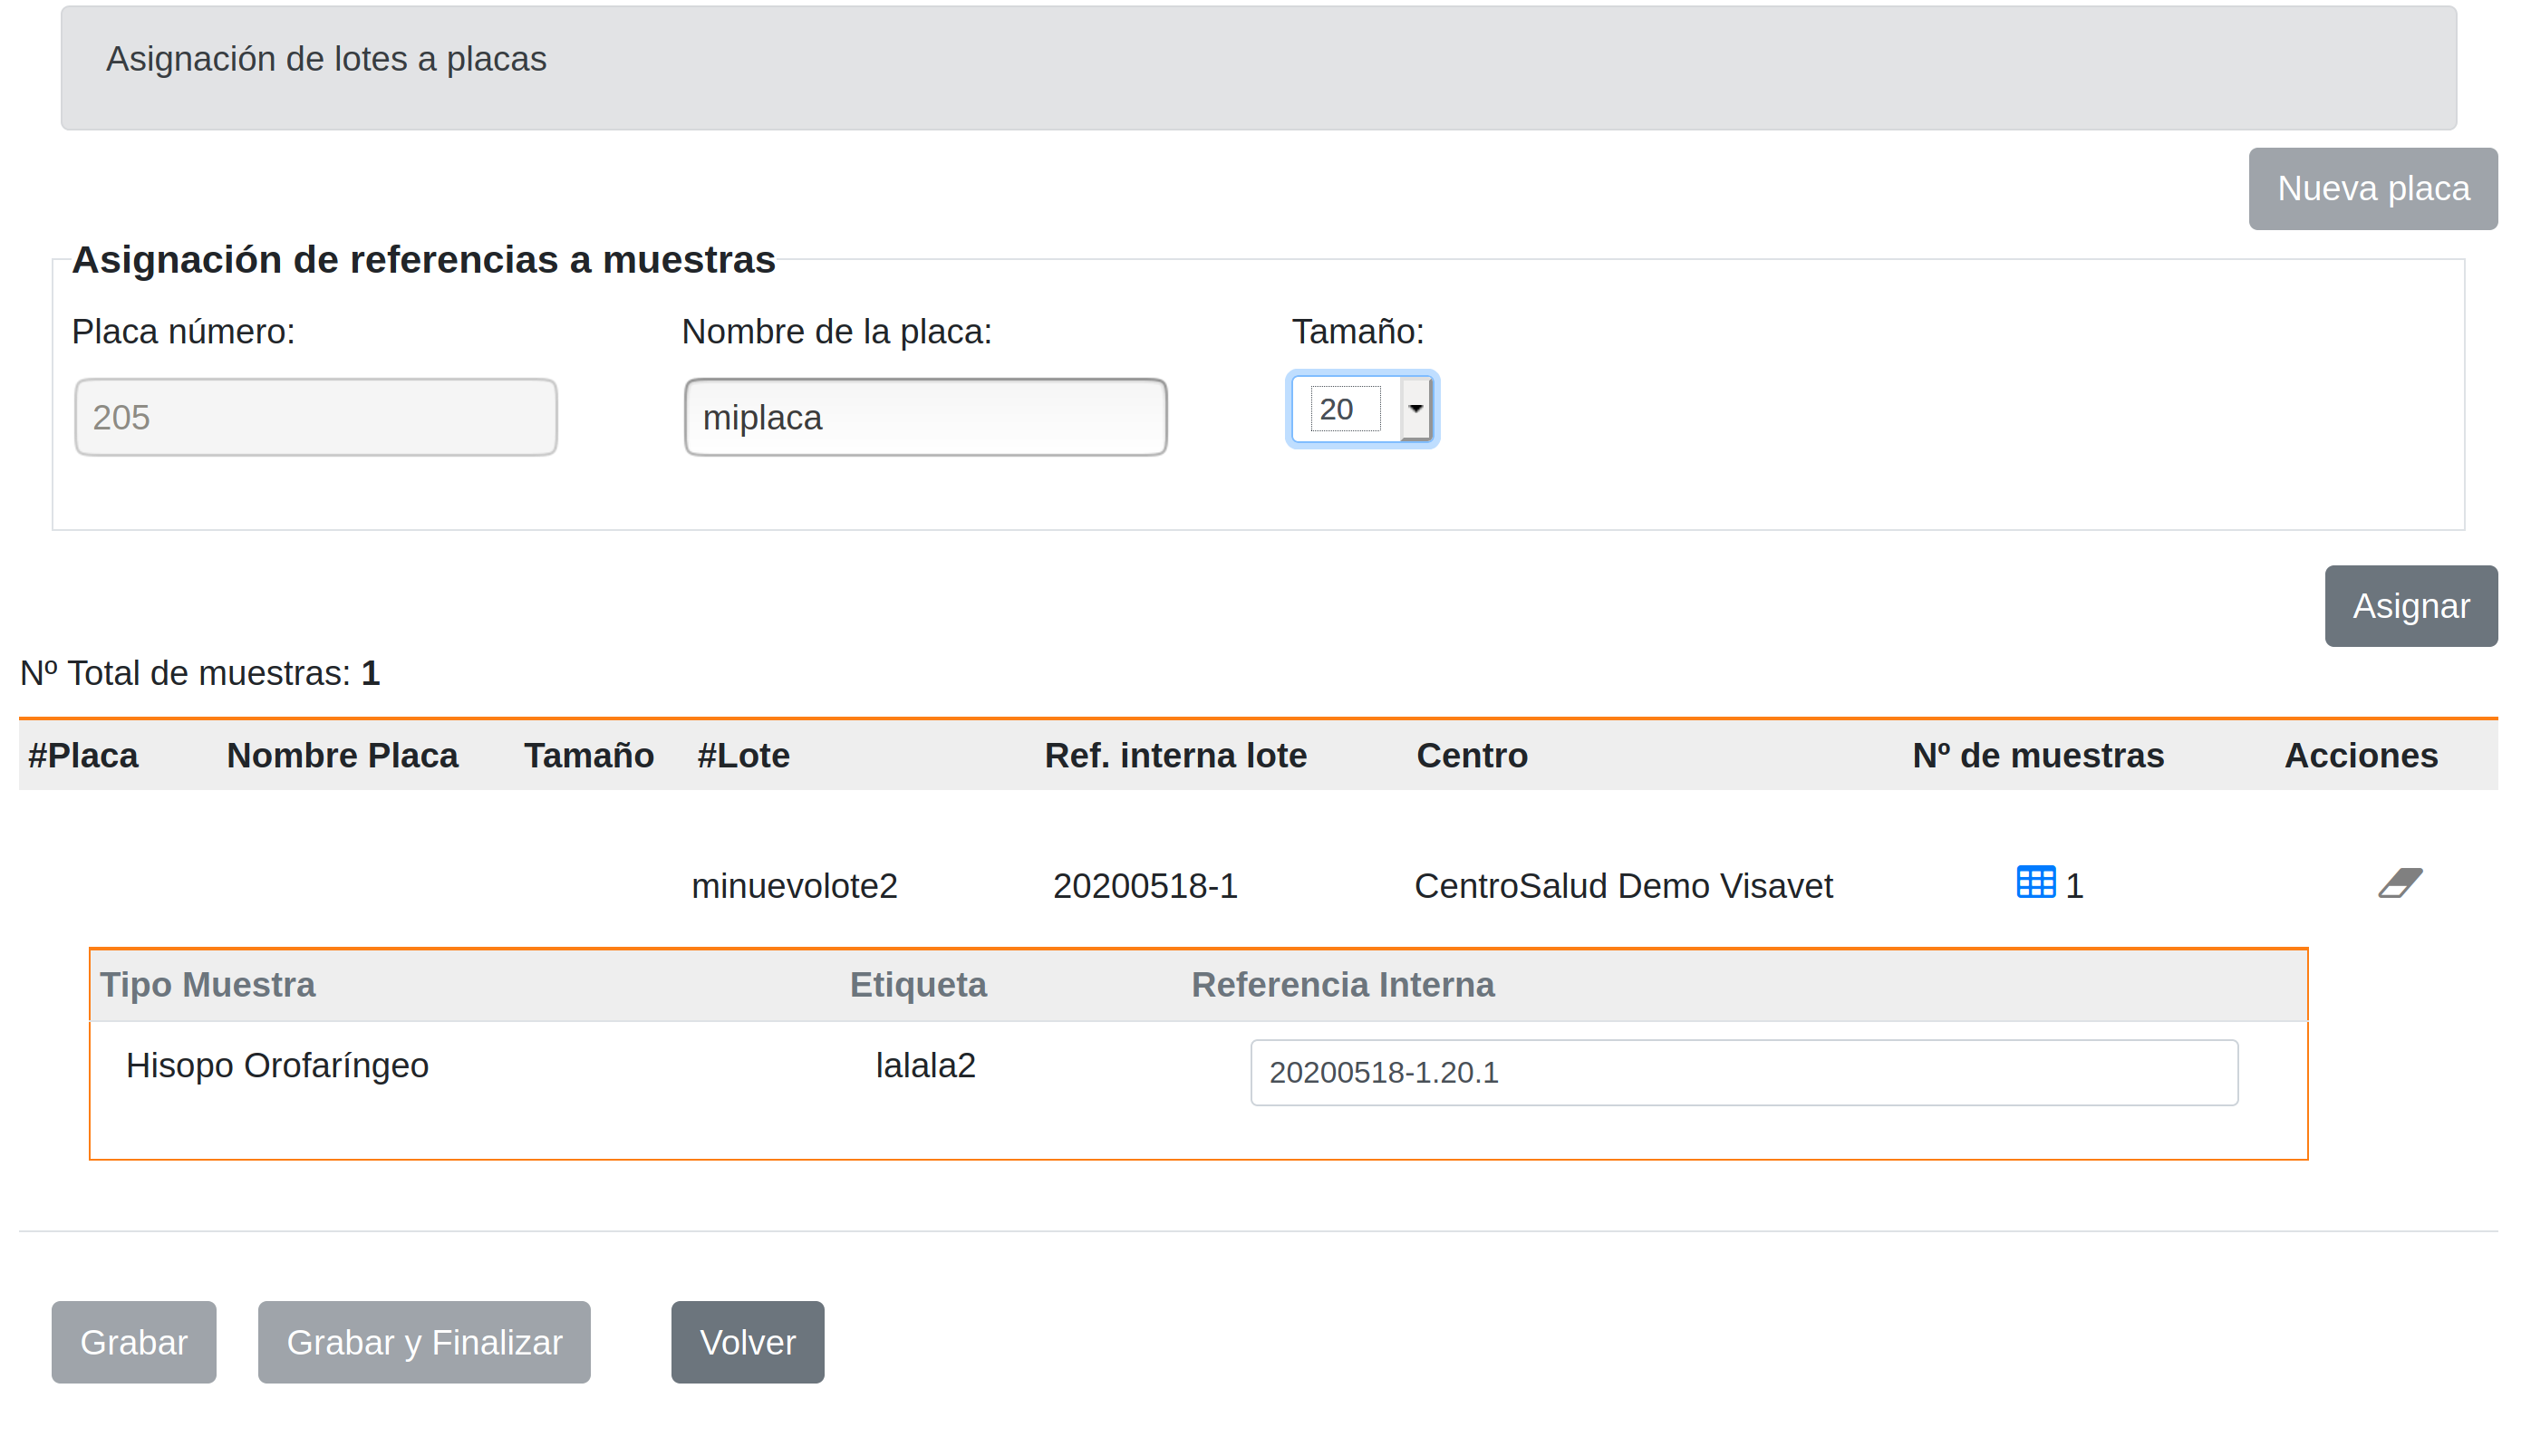
\includegraphics[width=0.7\textwidth]{Figs/Fig18.png}
\caption{Asignación de lotes a placas}
\label{Fig18}
\end{figure}

En esta pantalla, podremos proceder de la siguiente forma:

\begin{enumerate}
    \item Creando una nueva placa si no existe ninguna con capacidad disponible para las muestras a procesar. Para ello, daremos un nombre a la placa que la indentificará posteriormente en el laboratorio, e indicaremos su capacidad máxima en número de muestras.
    \item Verificaremos las muestras de nuestro lote y asignaremos una referencia interna que nos permite localizar la muestra en la placa PCR.
    \item Asignaremos la placa al lote haciendo click en el botón ASIGNAR.
    \item Una vez asignado todos los lotes a la placa, podremos GRABAR Y FINALIZAR.
\end{enumerate}

\subsection{Gestionar placas}

Dentro de esta pantalla podremos visualizar el estado, y gestionar las opciones de cada una de las placas PCR que se están procesando en el laboratorio. Para acceder al listado de placas, se puede hacer una búsqueda en función de los parámetros siguientes: laboratorio asignado, ID de placa, nombre de placa, fecha de creación, o estado.

\begin{figure}[h]
\centering
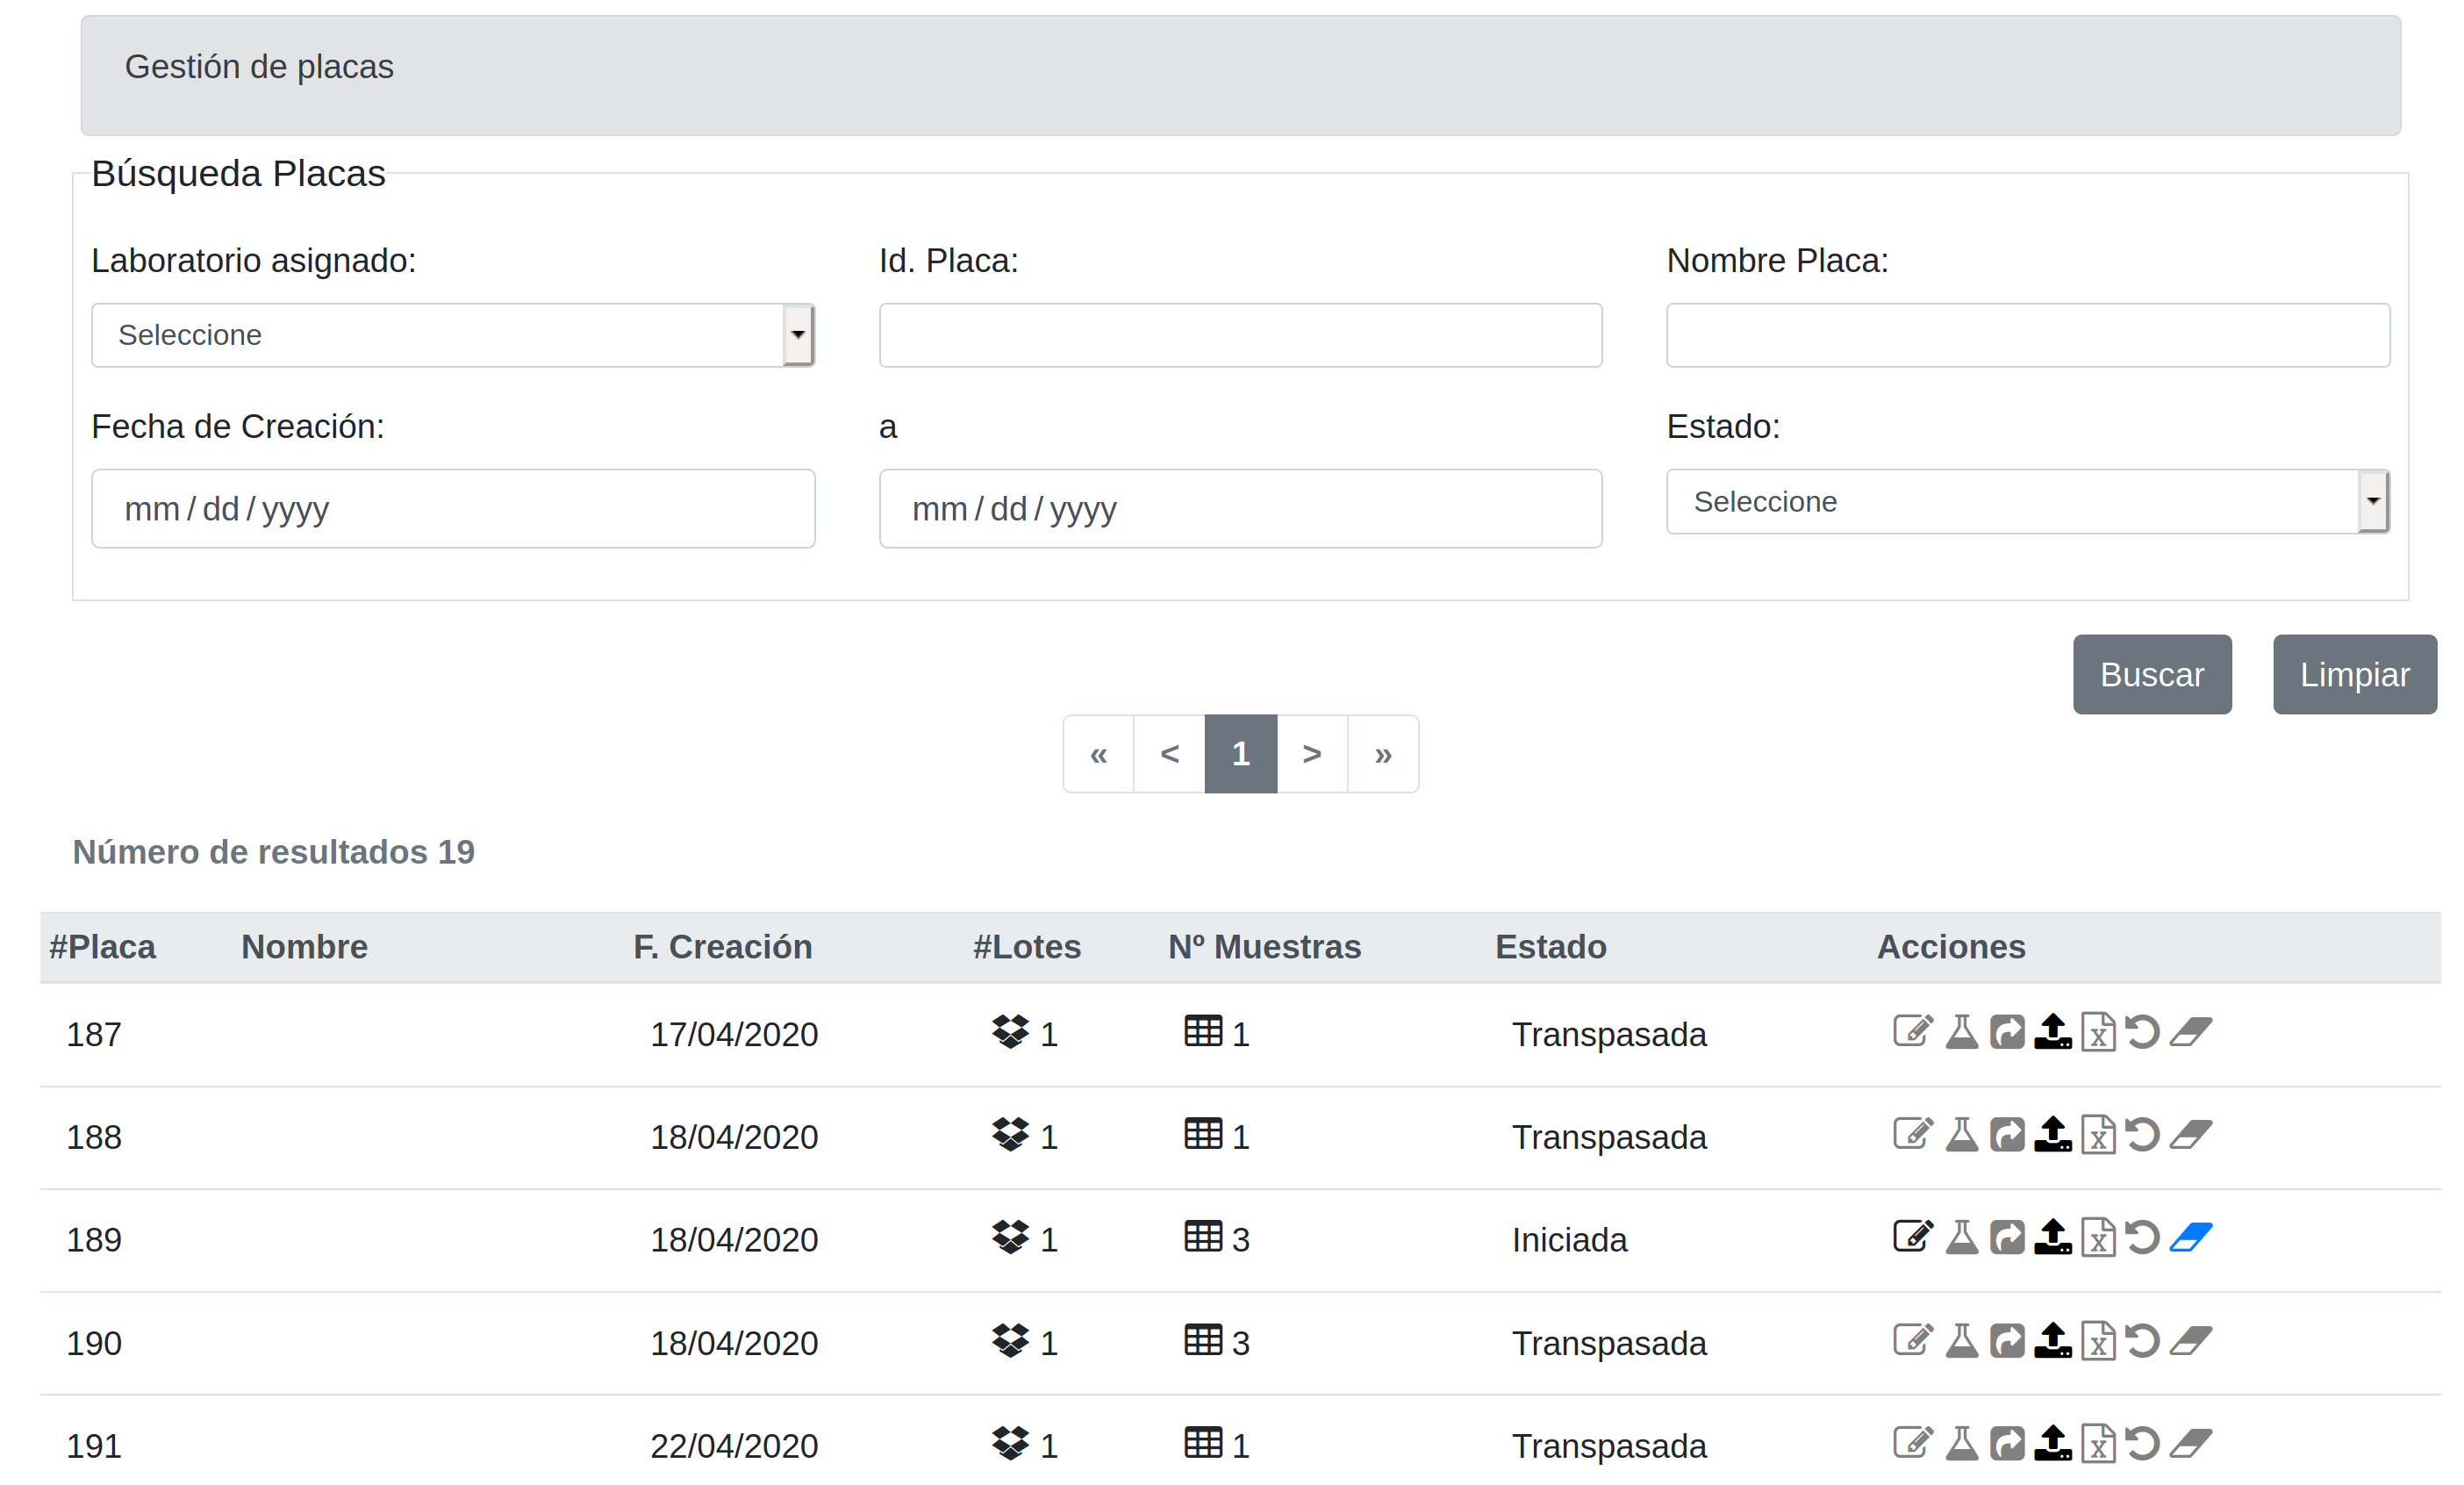
\includegraphics[width=0.7\textwidth]{Figs/Fig19.png}
\caption{Gestión de placas}
\label{Fig19}
\end{figure}

Dentro de este listado, podremos visualizar los datos de la placa:

\begin{itemize}
    \item nombre
    \item fecha de creación
    \item lotes dentro de la placa
    \item muestras en placa
    \item estado
\end{itemize}

Entre las opciones de gestión, tendremos la posibilidad de:

\begin{itemize}
    \item asignar laboratorio dentro del centro en el que procesaremos la placa
    
\begin{figure}[h]
\centering
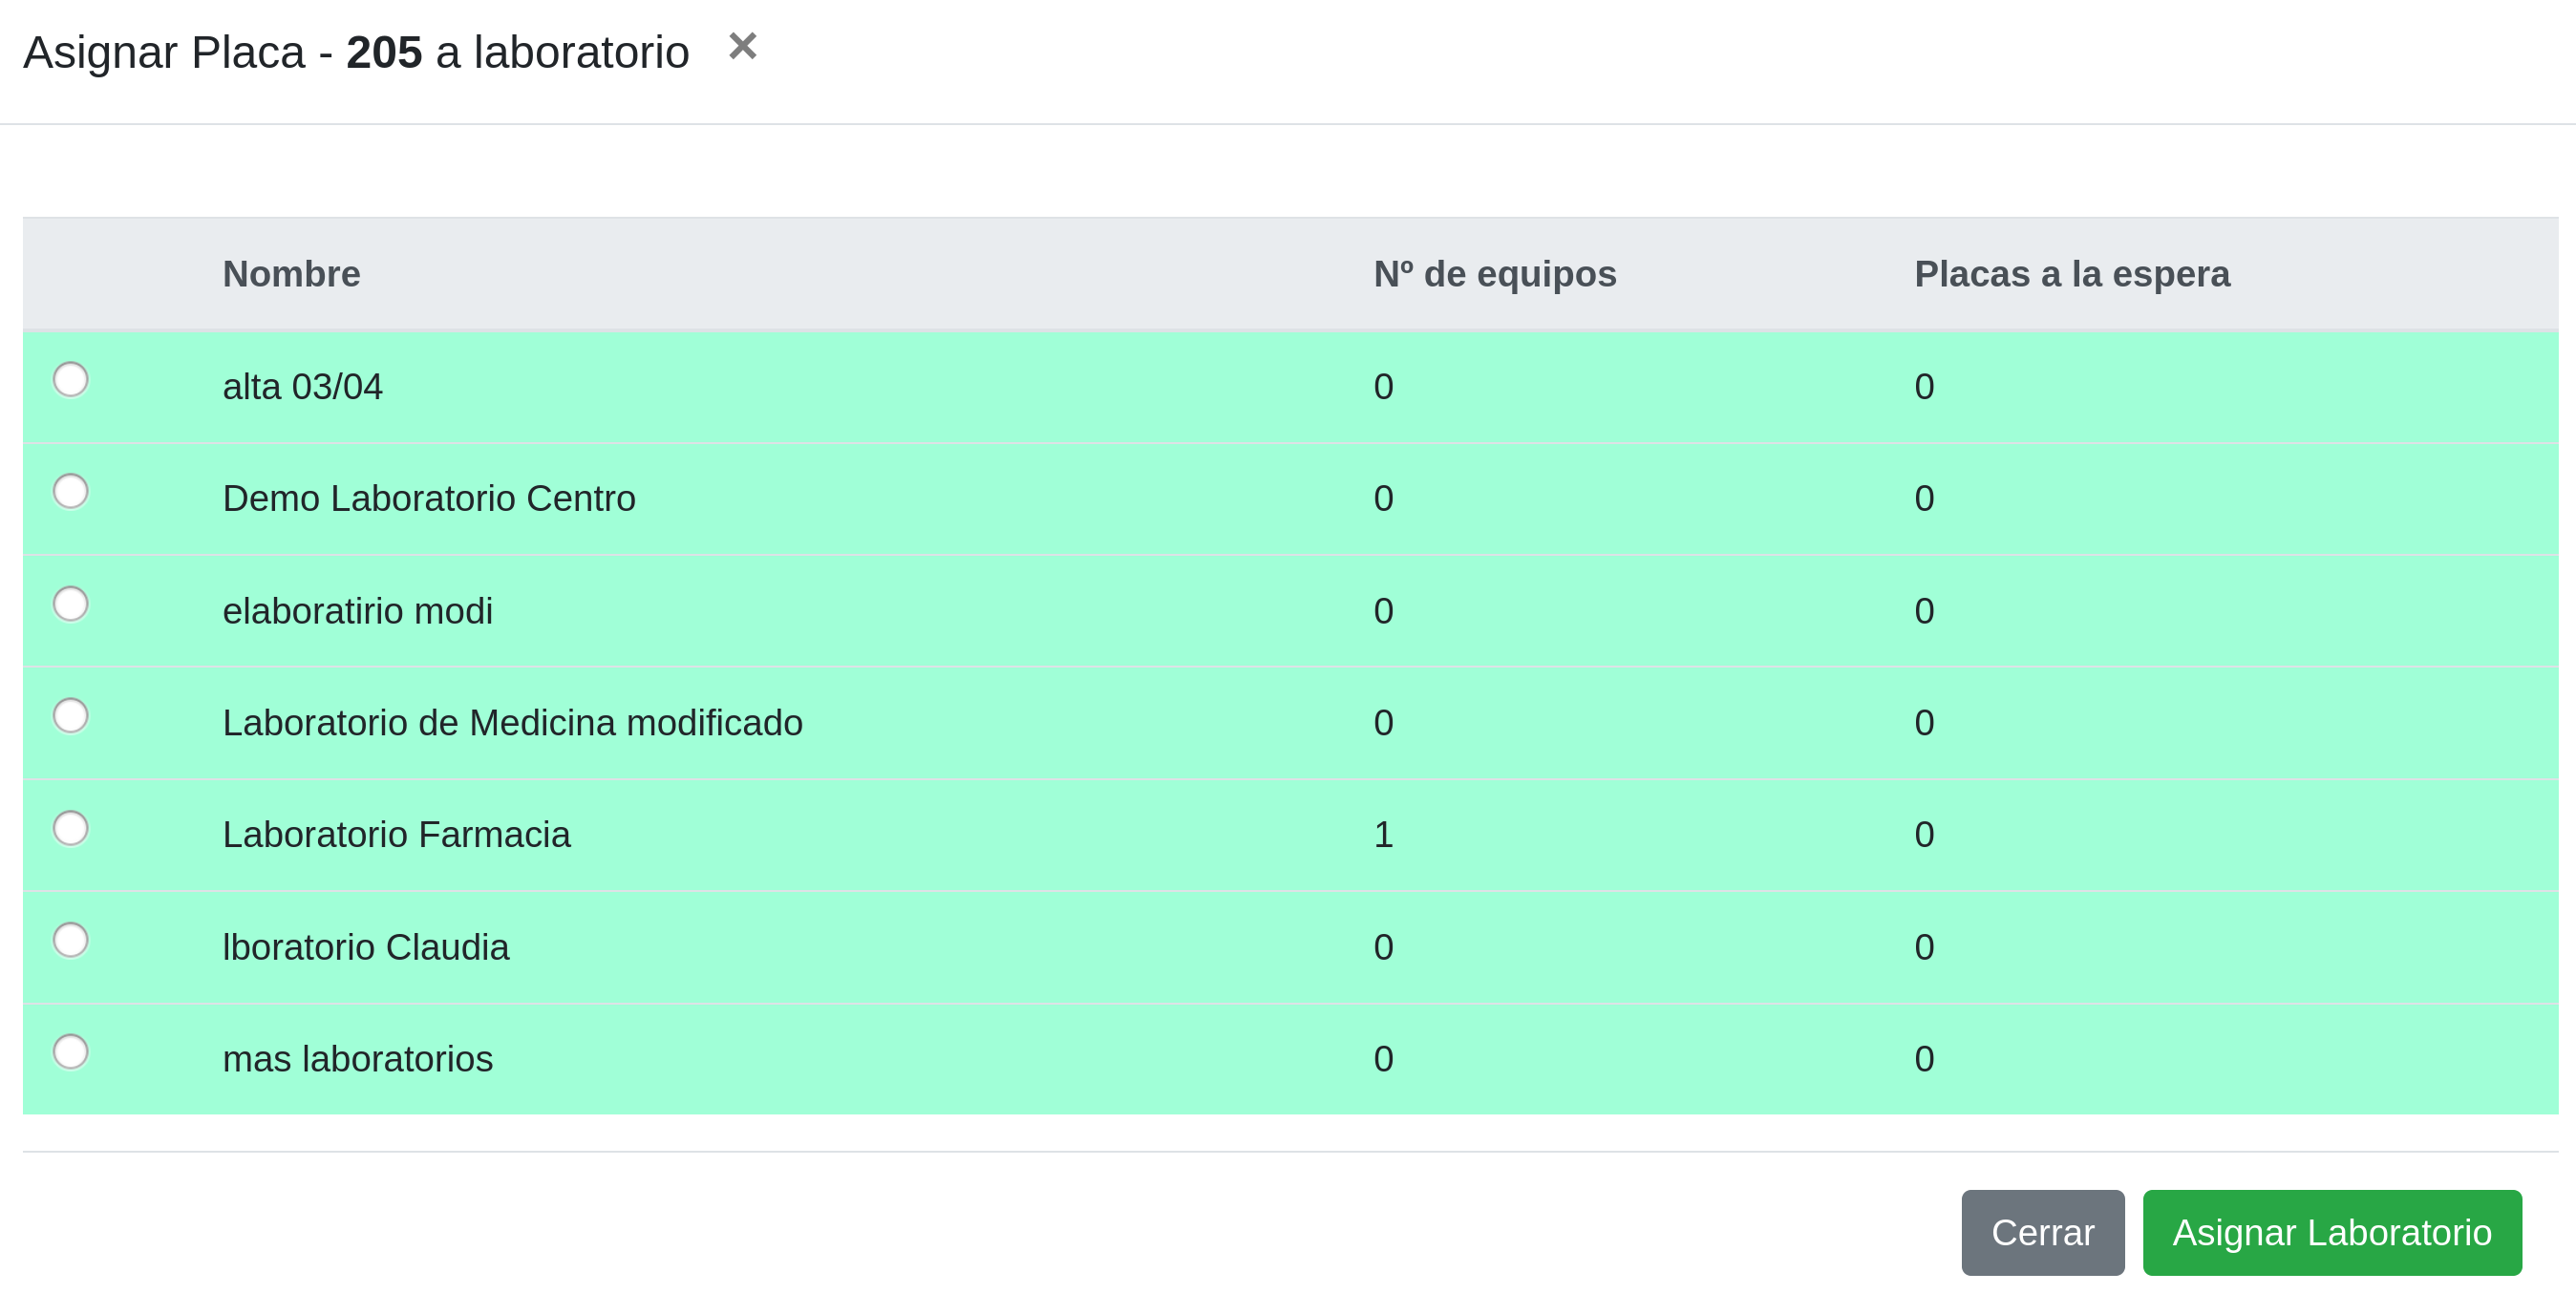
\includegraphics[width=0.7\textwidth]{Figs/Fig20.png}
\caption{Asignación de laboratorio}
\label{Fig20}
\end{figure}

    \item adjuntar documentación adicional a la placa si ésta lo requiere

\begin{figure}[h]
\centering
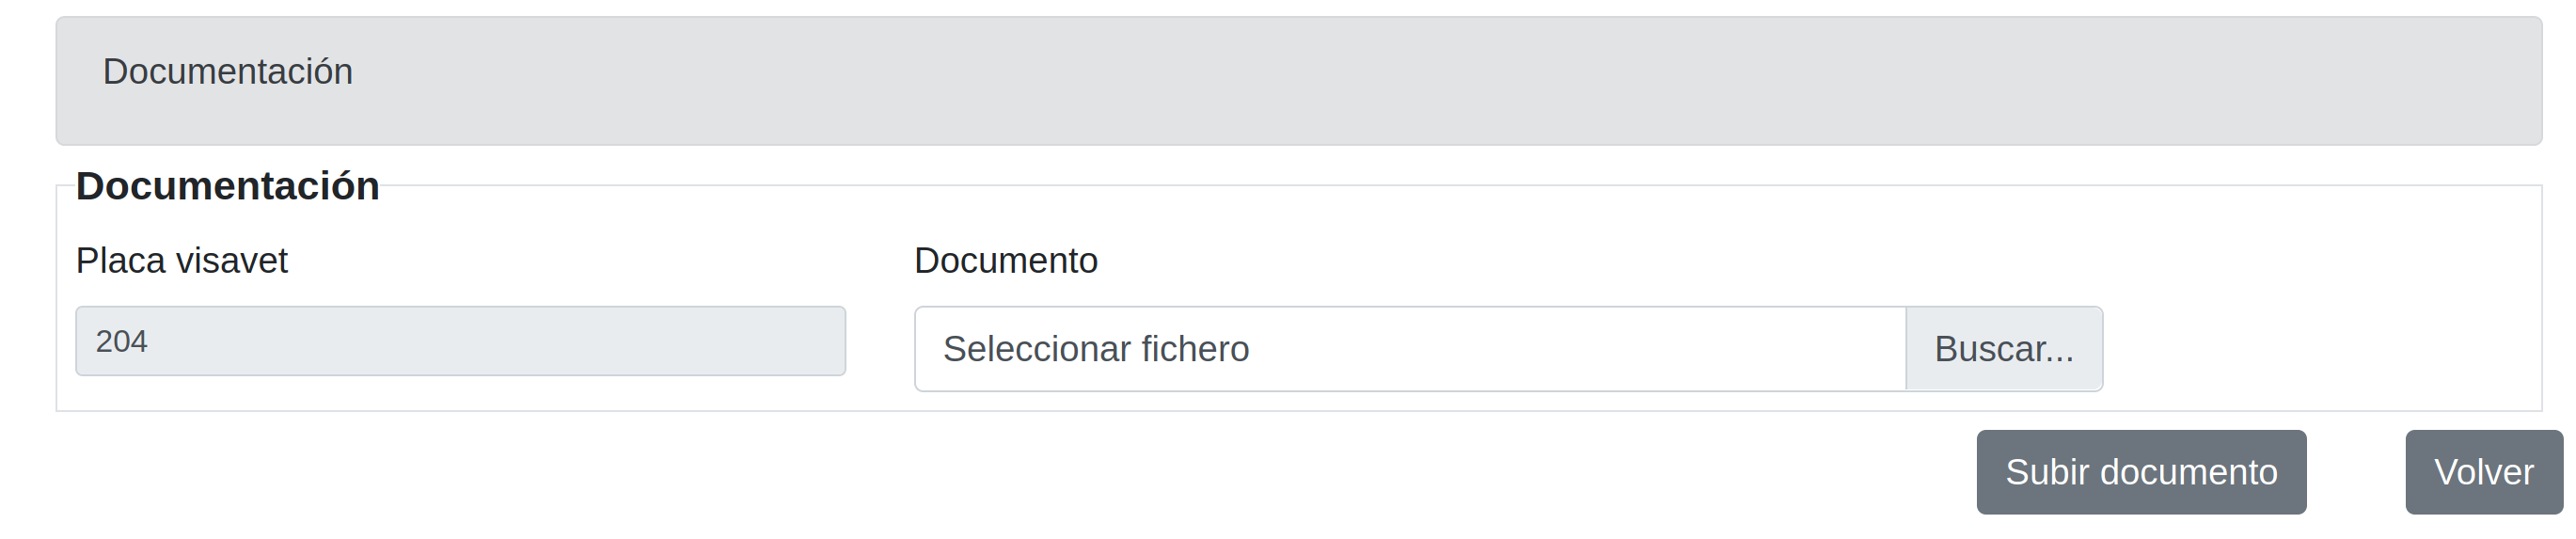
\includegraphics[width=0.7\textwidth]{Figs/Fig22.png}
\caption{Adjuntar documentación}
\label{Fig22}
\end{figure}

    \item una vez que el laboratorio ha sido seleccionado, podremos confirmar que la placa se traslada a éste para su procesamiento

\begin{figure}[h]
\centering
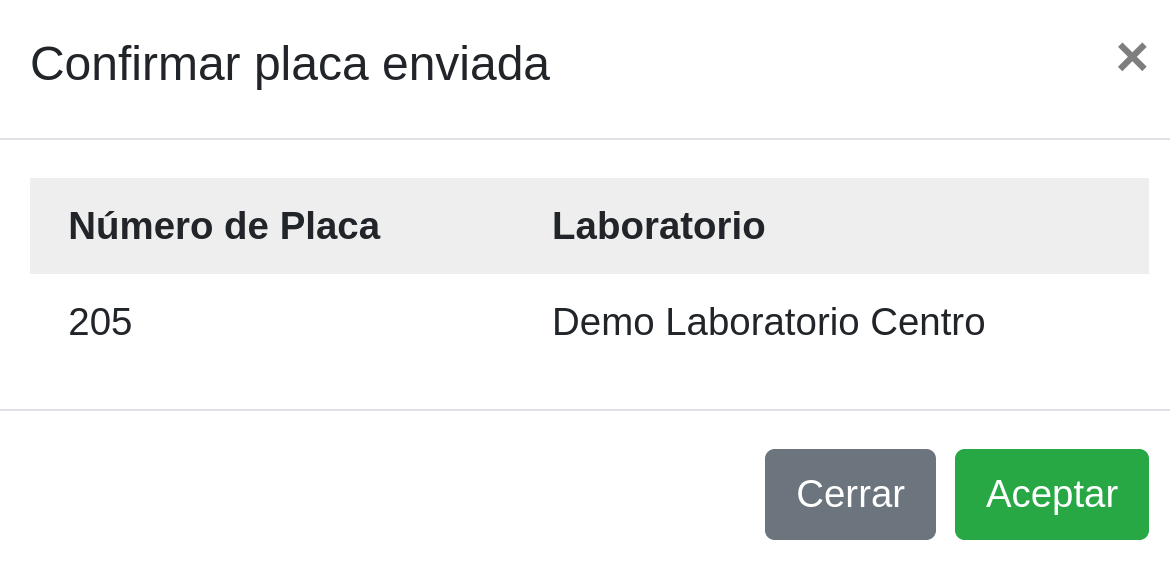
\includegraphics[width=0.5\textwidth]{Figs/Fig21.png}
\caption{Confirmar envío a laboratorio del centro}
\label{Fig21}
\end{figure}
    
\end{itemize}

\medskip
\begin{tcolorbox}[colback=blue!3!white,colframe=blue(ryb)!50!black,title=\textbf{Tip}]

Recordar que las placas deben trasladarse físicamente al laboratorio en el que éstas serán procesadas. Una vez trasladadas, confirmar el envío en la pantalla de gestión.

\end{tcolorbox}

\subsection{Carga sin datos previos del Centro de Salud}

En el caso de que las muestras...

\begin{figure}[h]
\centering
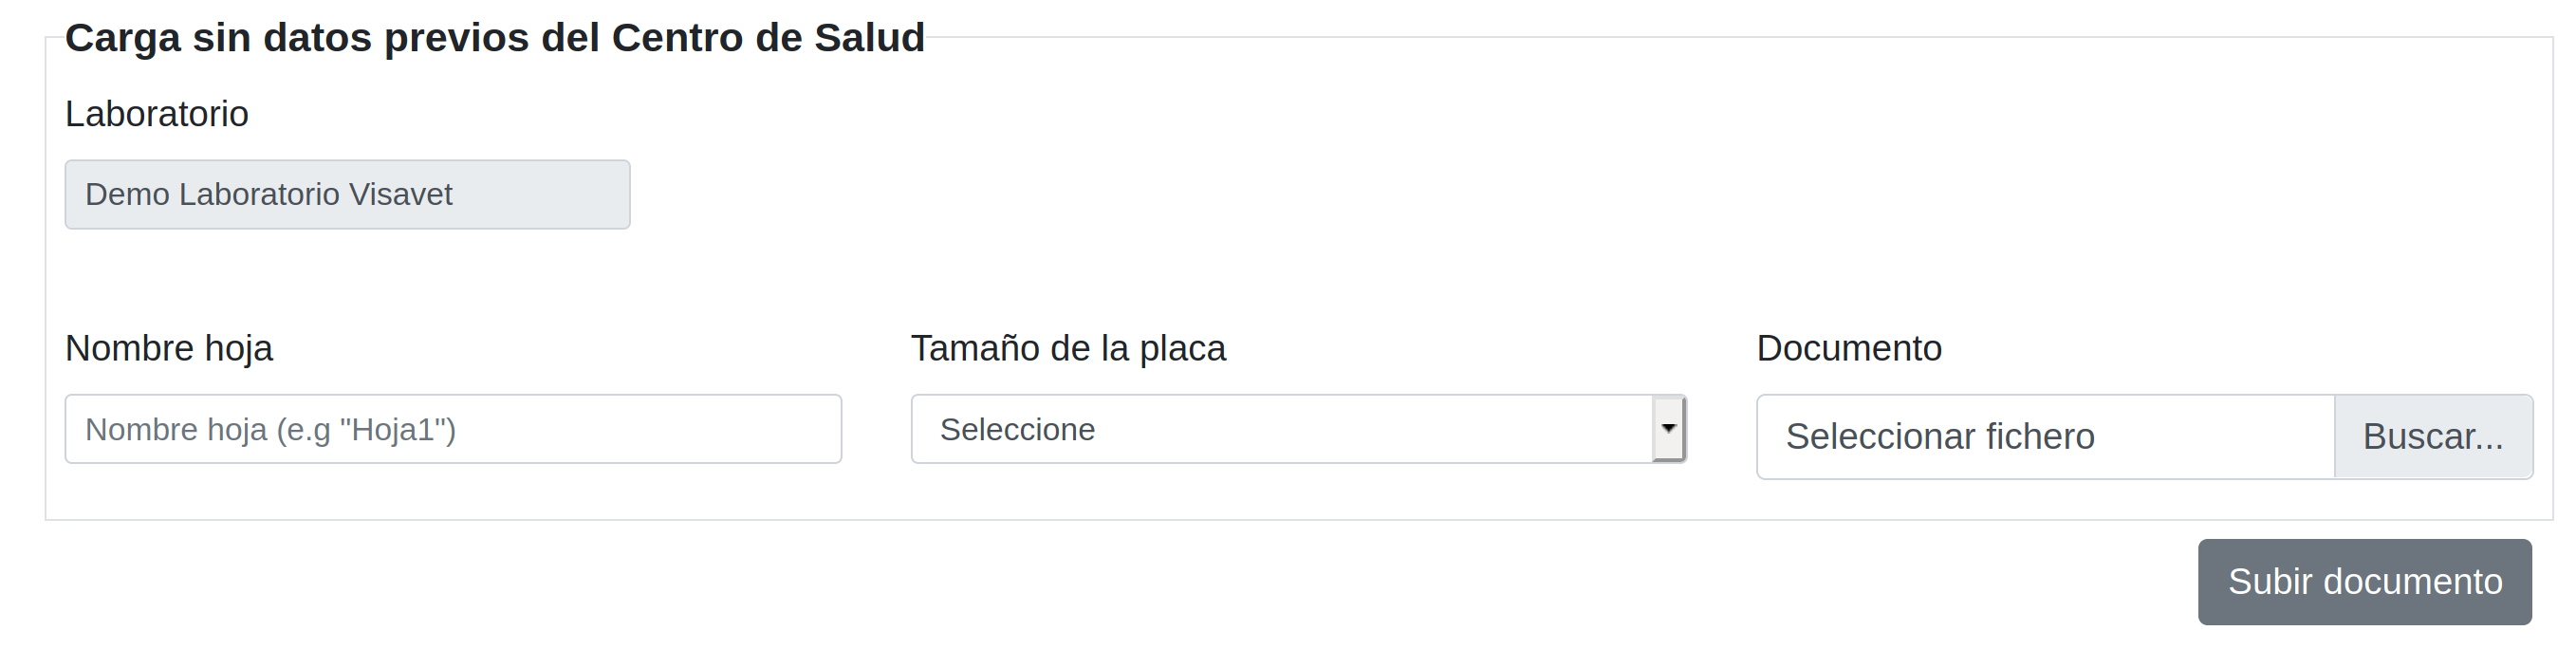
\includegraphics[width=0.7\textwidth]{Figs/Fig23.png}
\caption{Carga de datos de muestras}
\label{Fig23}
\end{figure}


%Beginning References. Don't add any text beyond this.
%------------------------------------------

\newpage %sending References to the last page

\bibliography{docu}
\bibliographystyle{apalike}
\end {document}